%%%%%%%%%%%%%%%%%%%%%%%%%%%%%%%%%%%%%%%%%%%%%%%%%%%%%%%%%%%%
%%  This Beamer template was created by Cameron Bracken.
%%  Anyone can freely use or modify it for any purpose
%%  without attribution.
%%
%%  Last Modified: January 9, 2009
%%

\documentclass[xcolor=x11names,compress]{beamer}

%% General document %%%%%%%%%%%%%%%%%%%%%%%%%%%%%%%%%%
\usepackage{graphicx}
\usepackage{tikz}
\usetikzlibrary{decorations.fractals}
%%%%%%%%%%%%%%%%%%%%%%%%%%%%%%%%%%%%%%%%%%%%%%%%%%%%%%

\usepackage{booktabs}


%% Beamer Layout %%%%%%%%%%%%%%%%%%%%%%%%%%%%%%%%%%
\useoutertheme[subsection=false,shadow]{miniframes}
\useinnertheme{default}
\usefonttheme{serif}
\usepackage{palatino}


\setbeamerfont{title like}{shape=\scshape}
\setbeamerfont{frametitle}{shape=\scshape}

\setbeamercolor*{lower separation line head}{bg=DeepSkyBlue4}
\setbeamercolor*{normal text}{fg=black,bg=white}
\setbeamercolor*{alerted text}{fg=red}
\setbeamercolor*{example text}{fg=black}
\setbeamercolor*{structure}{fg=black}

\setbeamercolor*{palette tertiary}{fg=black,bg=black!10}
\setbeamercolor*{palette quaternary}{fg=black,bg=black!10}

\renewcommand{\(}{\begin{columns}}
\renewcommand{\)}{\end{columns}}
\newcommand{\<}[1]{\begin{column}{#1}}
\renewcommand{\>}{\end{column}}
%%%%%%%%%%%%%%%%%%%%%%%%%%%%%%%%%%%%%%%%%%%%%%%%%%




\begin{document}


%%%%%%%%%%%%%%%%%%%%%%%%%%%%%%%%%%%%%%%%%%%%%%%%%%%%%%
%%%%%%%%%%%%%%%%%%%%%%%%%%%%%%%%%%%%%%%%%%%%%%%%%%%%%%
\section{\scshape Introduction}
\begin{frame}
\title{Reserve in Electricity Markets}
%\subtitle{SUBTITLE}
\author{
    Nigel Cleland\\
    {\it University of Auckland \\
    EPOC}\\
}
\date{

    \vspace{1cm}
    \today
}
\titlepage
\end{frame}

%%%%%%%%%%%%%%%%%%%%%%%%%%%%%%%%%%%%%%%%%%%%%%%%%%%%%%
%%%%%%%%%%%%%%%%%%%%%%%%%%%%%%%%%%%%%%%%%%%%%%%%%%%%%%
\begin{frame}{Introduction}
\tableofcontents
\end{frame}

\begin{frame}{About Me}
\begin{itemize}
\item University of Canterbury, BE(Hons) Chemical and Process Engineering
\item University of Auckland, Year Three, Ph.D Eng. Sci and C\&M
\item Prior work at load aggregators
\item HVDC Pole 3 Commissioning (Trading Team)
\item Based at Transpower S.O. 2013
\item Various Consulting Jobs
\end{itemize}
\end{frame}


%%%%%%%%%%%%%%%%%%%%%%%%%%%%%%%%%%%%%%%%%%%%%%%%%%%%%%
%%%%%%%%%%%%%%%%%%%%%%%%%%%%%%%%%%%%%%%%%%%%%%%%%%%%%%
\section{\scshape Reserve Constraints}
\begin{frame}
\vspace{1.5cm}
\begin{center}
{\Huge\textit{Reserve Constraints}}
\end{center}
\end{frame}

\begin{frame}{\scshape It starts with a picture}
\begin{figure}
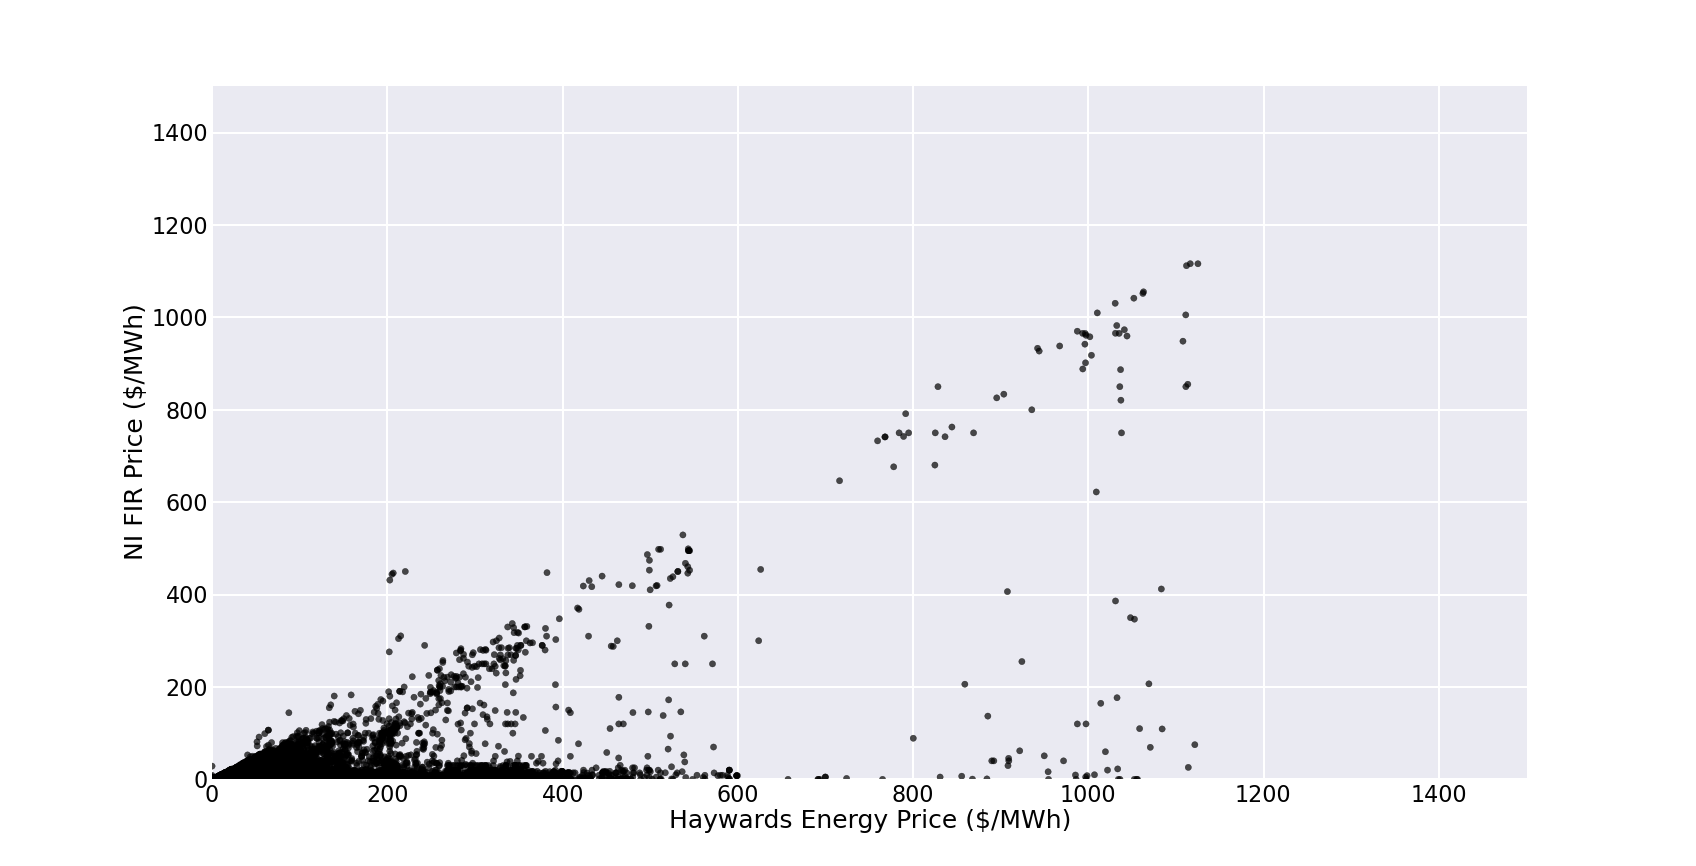
\includegraphics[width=0.95\textwidth]{img/haywards_vs_ni_fir.png}
\caption{Haywards Nodal Spot Price (x axis) compared with the North Island
FIR Price (y axis)}
\end{figure}
\end{frame}

%%%%%%%%%%%%%%%%%%%%%%%%%%%%%%%%%%%%%%%%%%%%%%%%%%%%%%
%%%%%%%%%%%%%%%%%%%%%%%%%%%%%%%%%%%%%%%%%%%%%%%%%%%%%%
\begin{frame}{\scshape Why does this matter?}
\begin{figure}
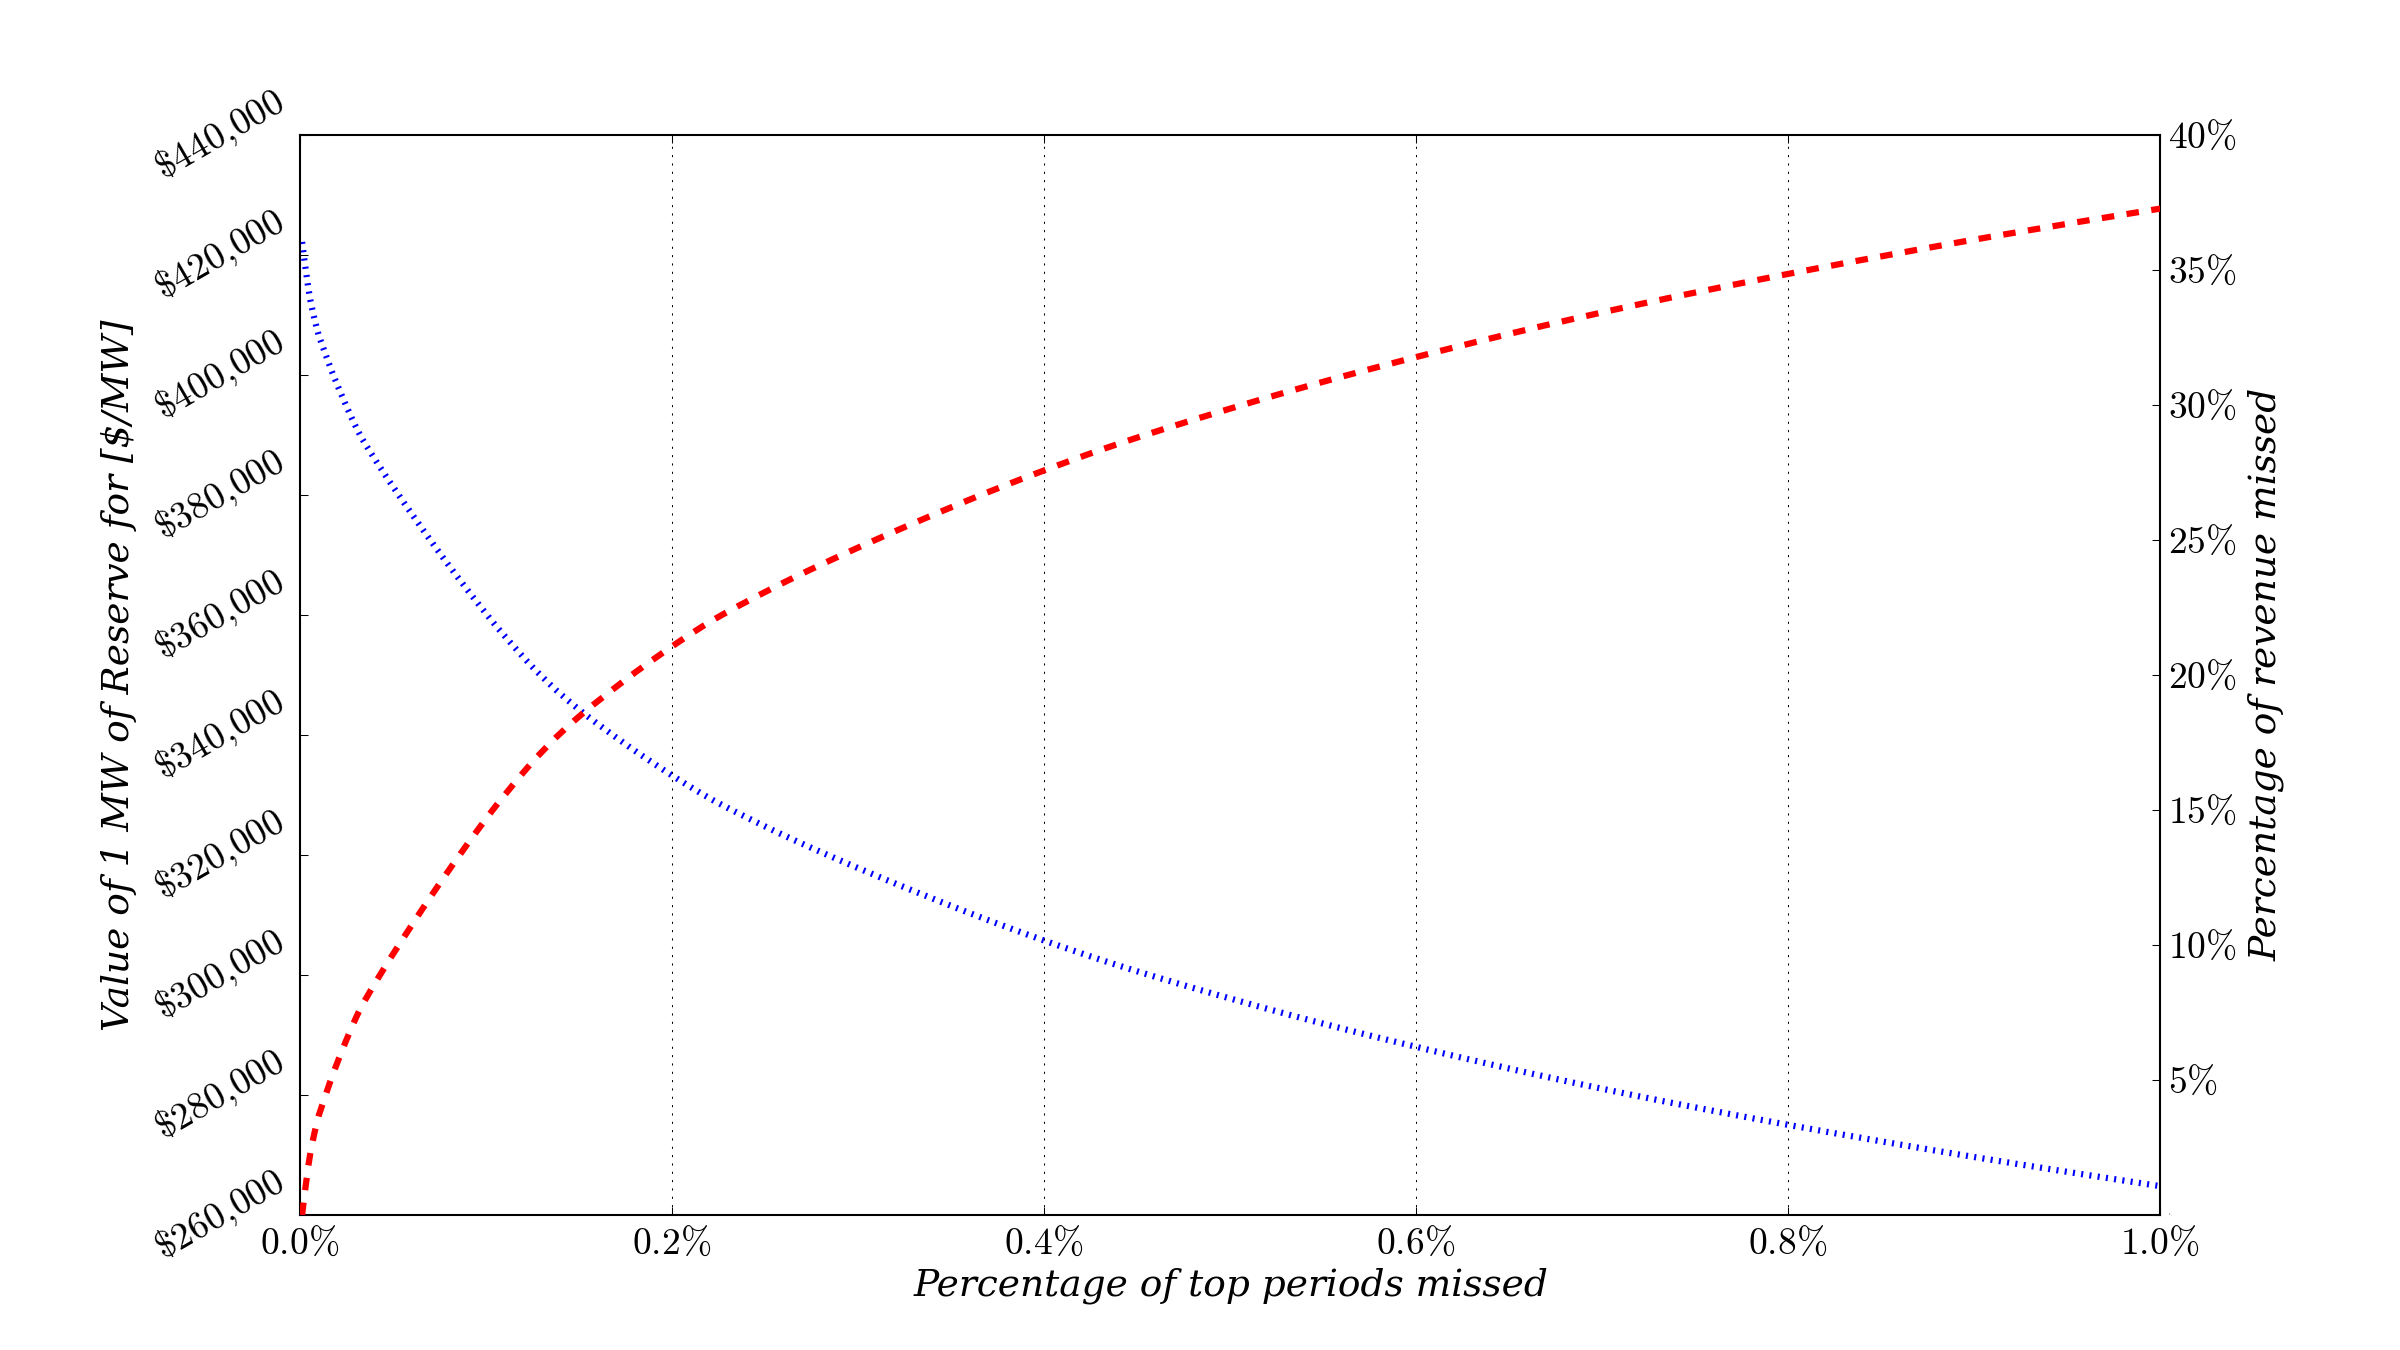
\includegraphics[width=0.95\textwidth]{img/reserveprice.png}
\caption{Revenue ``lost'' for missing highly priced trading periods}
\end{figure}
\end{frame}

\begin{frame}{\scshape Effect on Individual Consumers}
\begin{table}
\caption{Monthly Revenue ``missed'' by various IL producers}
\begin{tabular}{cccc}
\toprule
& NZST & PPAC & SKOG \\
\midrule
2009 & 18-85\% & 2-92\% & 30-80\% \\
2010 & 4-90\% & 0-90\% & 5-70\% \\
\bottomrule
\end{tabular}
\end{table}
In November 2010 NZST missed 90\% of the monthly IR Revenue, SKOG missed 6\%
\vspace{2cm}
\end{frame}

%%%%%%%%%%%%%%%%%%%%%%%%%%%%%%%%%%%%%%%%%%%%%%%%%%%%%%
%%%%%%%%%%%%%%%%%%%%%%%%%%%%%%%%%%%%%%%%%%%%%%%%%%%%%%
\begin{frame}{\scshape Some Theory}
\scalebox{0.75}{
\begin{minipage}{0.50\textwidth}
\begin{eqnarray*}
[POPF] \min & p_g^T g + p_r^T r & \\
\text{st.} &  Mg + Af = d &[\pi] \\
                  &  r + g \le G &[\epsilon] \\
                  &  r - Kg \le 0 &[\kappa]  \\
                  & Er - g \ge 0 &[\lambda^{1}] \\
                  & Hr - Bf \ge 0 &[\lambda^{2}] \\
                  & r \le R &[\omega] \\
                  & |f| \le F &[\tau^{\pm}] \\
                  & Lf  = 0 & [\alpha] \\
                  & r, g \geq 0 & \\
\end{eqnarray*}
\end{minipage}}
\scalebox{0.75}{
\begin{minipage}{0.3\textwidth}
\begin{eqnarray*}
[DOPF] \max & d^{T} + R^{T}\omega + G^{T}\epsilon + F^{T}(\tau^{+} +
\tau^{-}) & \\
\text{st.} & M^{T}\pi + \epsilon - K\kappa + \lambda^{1} \le p_g &[g] \\
                  & \omega + \epsilon + \kappa + E\lambda^{1} \le p_r &[r]  \\
                  & A^{T}\pi + \tau^{+} - \tau^{-} - B^{T}\lambda^{2} +L^{T}\alpha = 0  &[f] \\
                  & \omega, \epsilon, \tau^{\pm}, \kappa \le 0 & \\
                  & \lambda^{1}, \lambda^{2} \ge 0 & \\
                  & & \\
                  & & \\
                  & & \\
                  & & \\
\end{eqnarray*}
\end{minipage}}
\end{frame}

\begin{frame}{\scshape Case Studies}
\begin{figure}
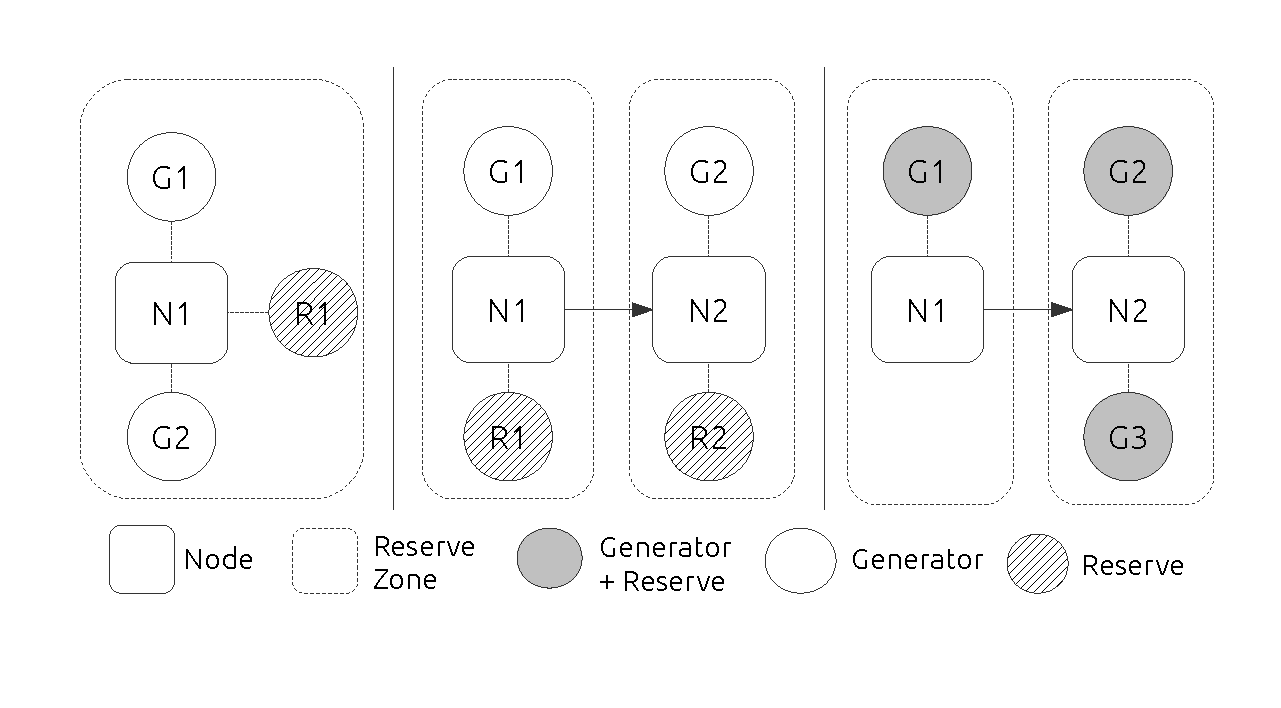
\includegraphics[width=0.95\textwidth]{img/nodal_diagram.pdf}
\caption{Some Case Studies to illustrate different mechanisms of binding
constraints occurring}
\end{figure}
\end{frame}


%%%%%%%%%%%%%%%%%%%%%%%%%%%%%%%%%%%%%%%%%%%%%%%%%%%%%%
%%%%%%%%%%%%%%%%%%%%%%%%%%%%%%%%%%%%%%%%%%%%%%%%%%%%%%
\begin{frame}{\scshape Case Study Results}
Marginal Risk Setting Generator
\begin{equation}
\pi = p_{g,marginal} - \lambda
\end{equation}
Risk Constrained Transmission Line
\begin{equation}
\pi_2 = \pi_1 - \lambda_2
\end{equation}
Bathtub Constrained Transmission
\begin{equation}
\pi_2 = \dfrac{1}{1+k_{g,2}}p_{g,2} + \dfrac{k_{g,2}}{1+k_{g,2}}(\pi_1 + \lambda_{2})
\end{equation}
\end{frame}

\begin{frame}{Testing These, Marginal Generator}
\begin{figure}
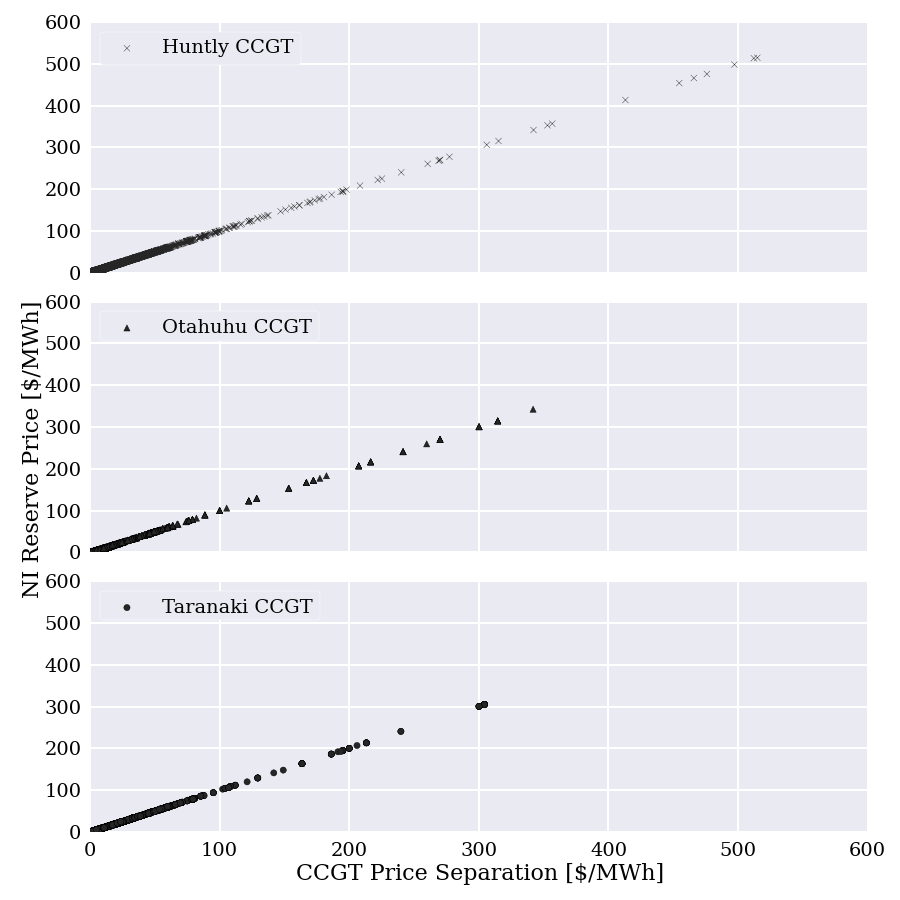
\includegraphics[scale=0.3]{img/ccgt_reserve_prices_offer_prices.png}
\caption{Reserve Constraints binding upon major CCGT Units}
\end{figure}
\end{frame}

\begin{frame}{Testing These, Marginal Transmission, NI}
\begin{figure}
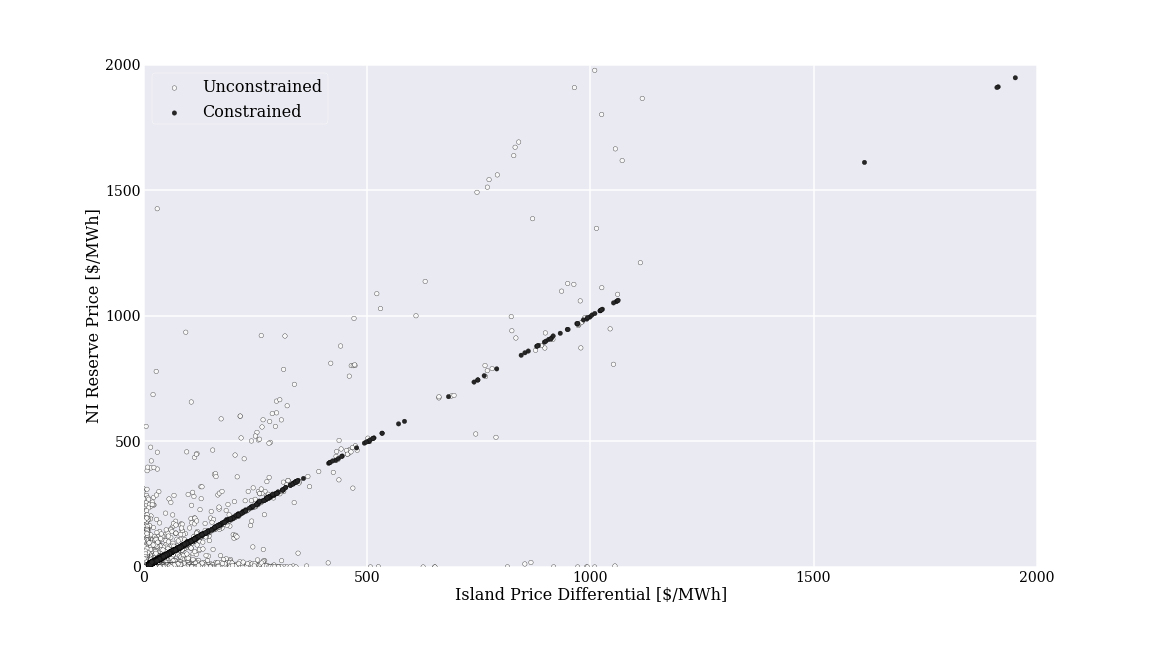
\includegraphics[width=0.95\textwidth]{img/ni_reserve_prices_island_differential.png}
\caption{Reserve Constraints Binding upon Northward HVDC Transmission}
\end{figure}
\end{frame}

\begin{frame}{Testing These, Marginal Transmission, SI}
\begin{figure}
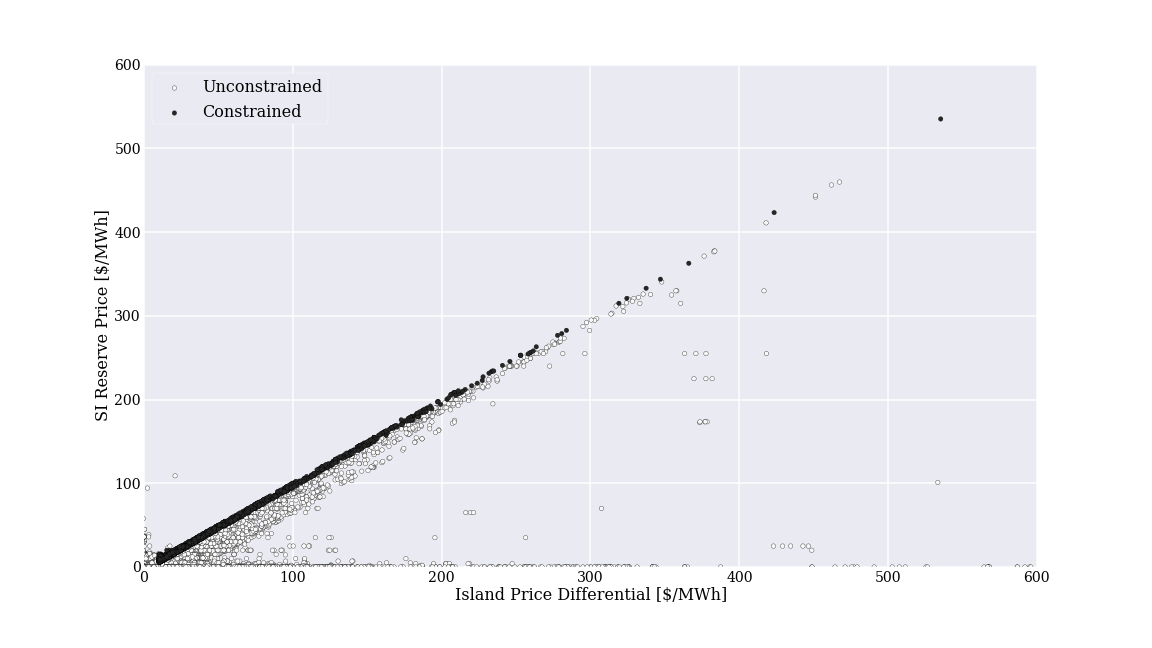
\includegraphics[width=0.95\textwidth]{img/si_reserve_prices_island_differential.png}
\caption{Reserve Constraints Binding upon Southward HVDC Transmission}
\end{figure}
\end{frame}

\begin{frame}{Testing These, Bathtub Constraints}
\begin{figure}
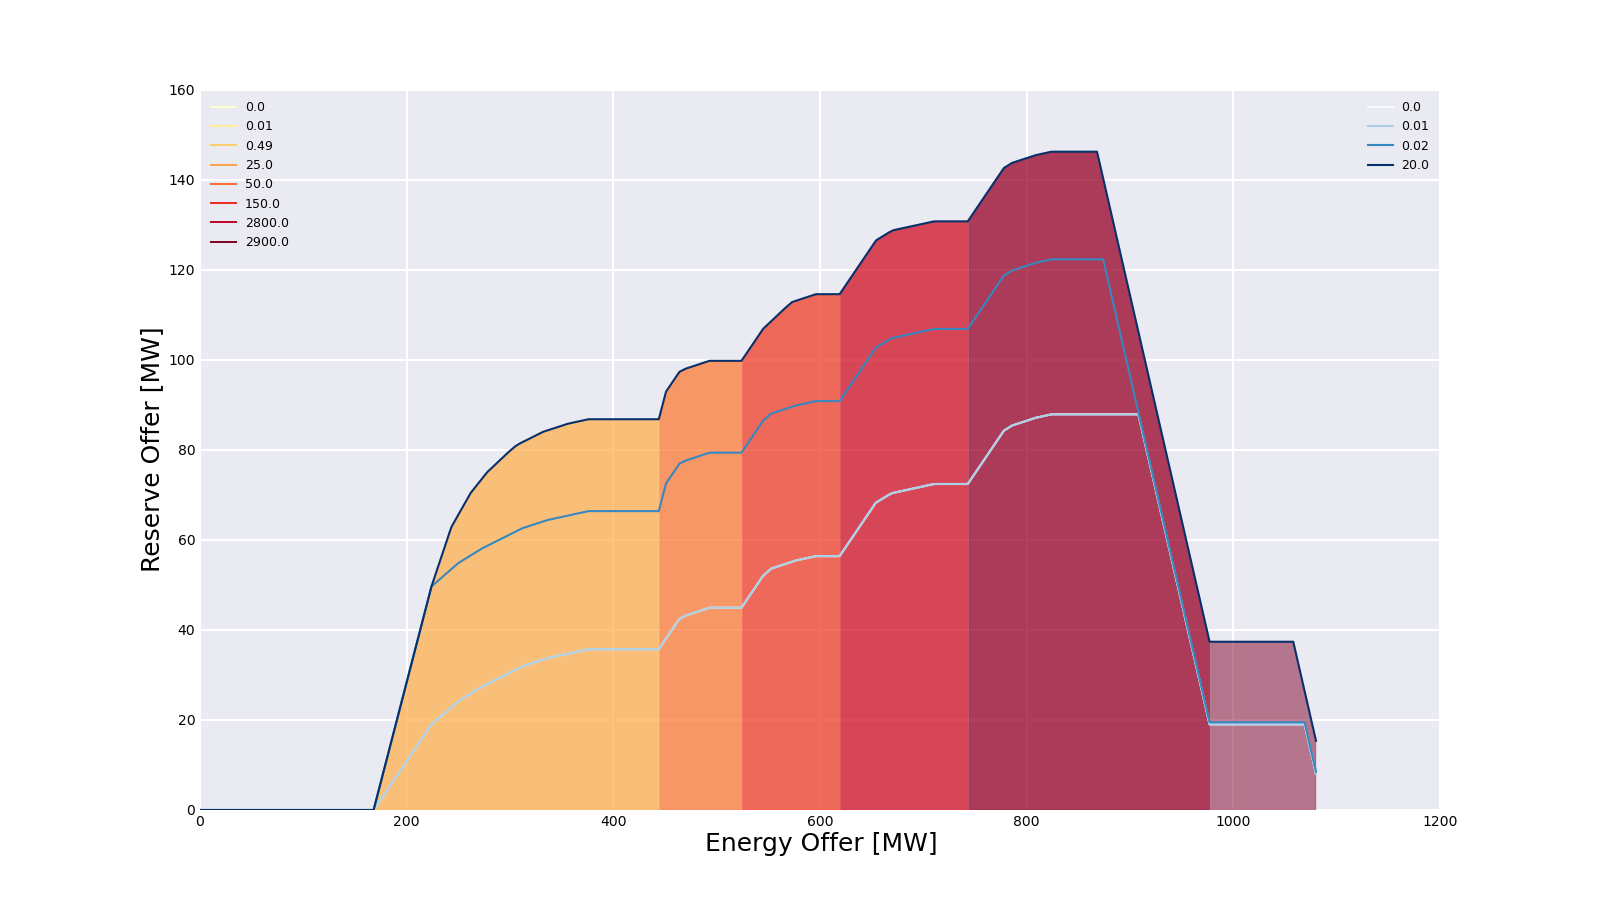
\includegraphics[width=0.95\textwidth]{img/mrpl_fan_curve.png}
\caption{Mighty River Fan Curve, TP 19, October 3 2013.}
\end{figure}
\end{frame}

\section{\scshape Spot Market Prices}
\begin{frame}
\vspace{1.5cm}
\begin{center}
{\Huge\textit{Spot Market Prices}}
\end{center}
\end{frame}

\begin{frame}{Scarcity, Constraints or Both?}
\begin{itemize}
\item How do we understand Price?
\item Moving up a merit order stack?
\item High Demand = High Price?
\item Hydrology? Price = f(Inverse Hydro)
\item Constraints?
\end{itemize}
\end{frame}

\begin{frame}{Average Price at Different Demand}
\begin{figure}
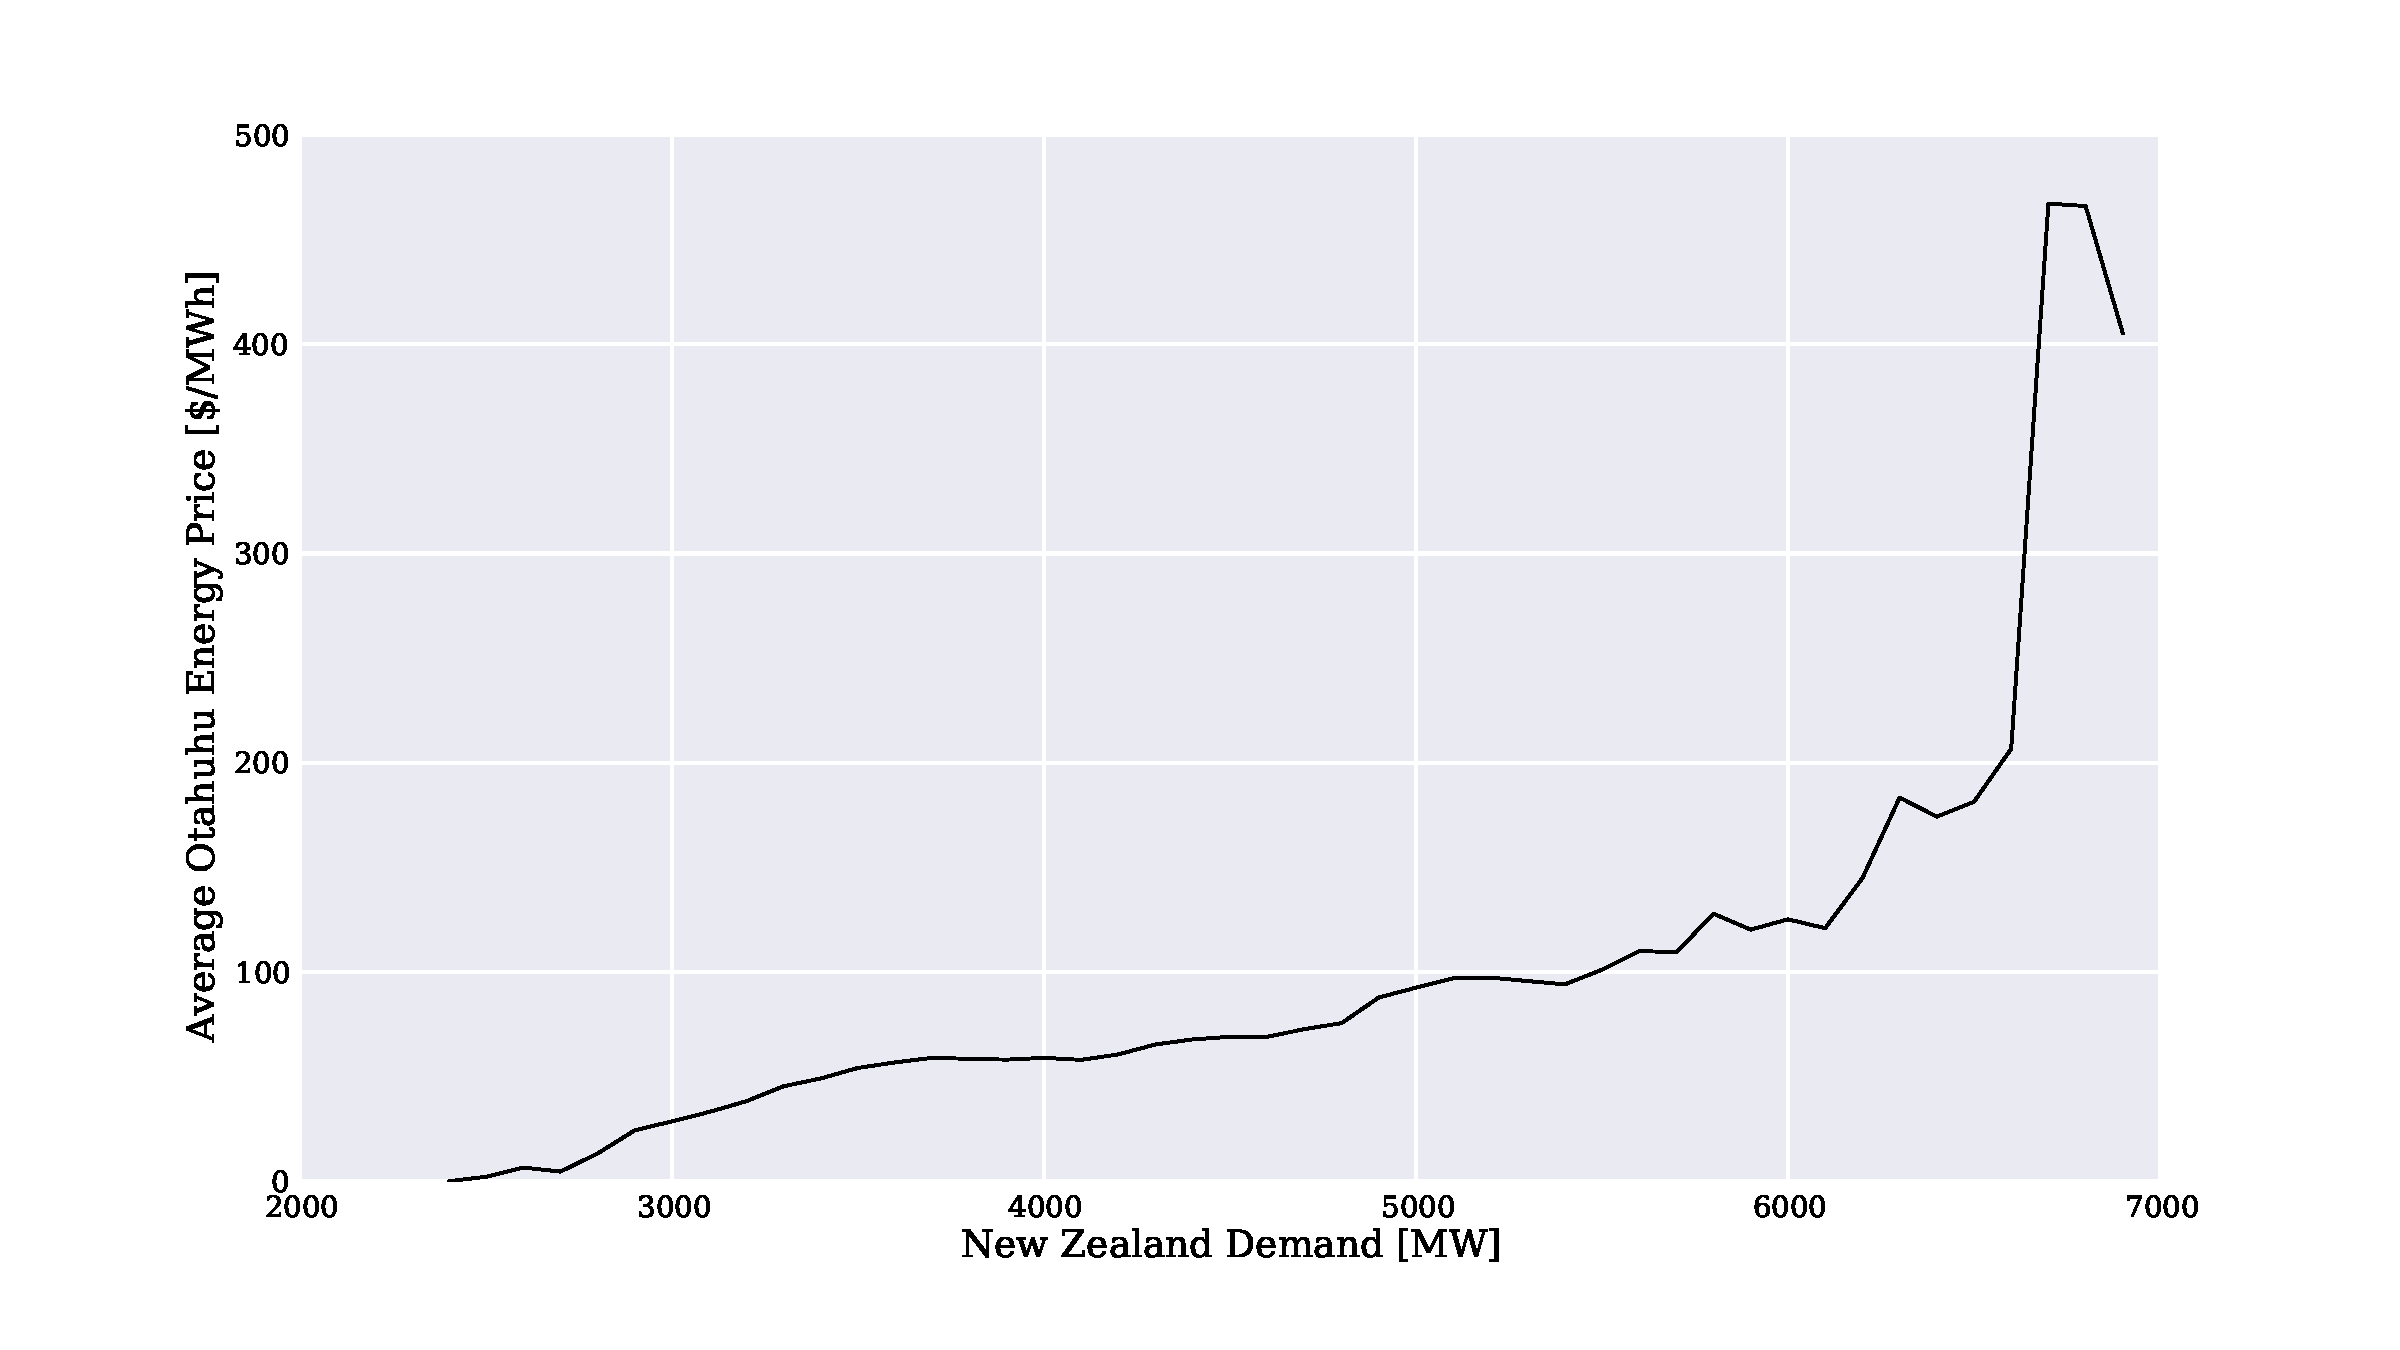
\includegraphics[width=0.95\textwidth]{img/price_vs_demand.pdf}
\caption{The higher the demand, the higher the energy price, we're moving up
the stack.}
\end{figure}
\end{frame}

\begin{frame}{Average Price at Different Hydrology}
\begin{figure}
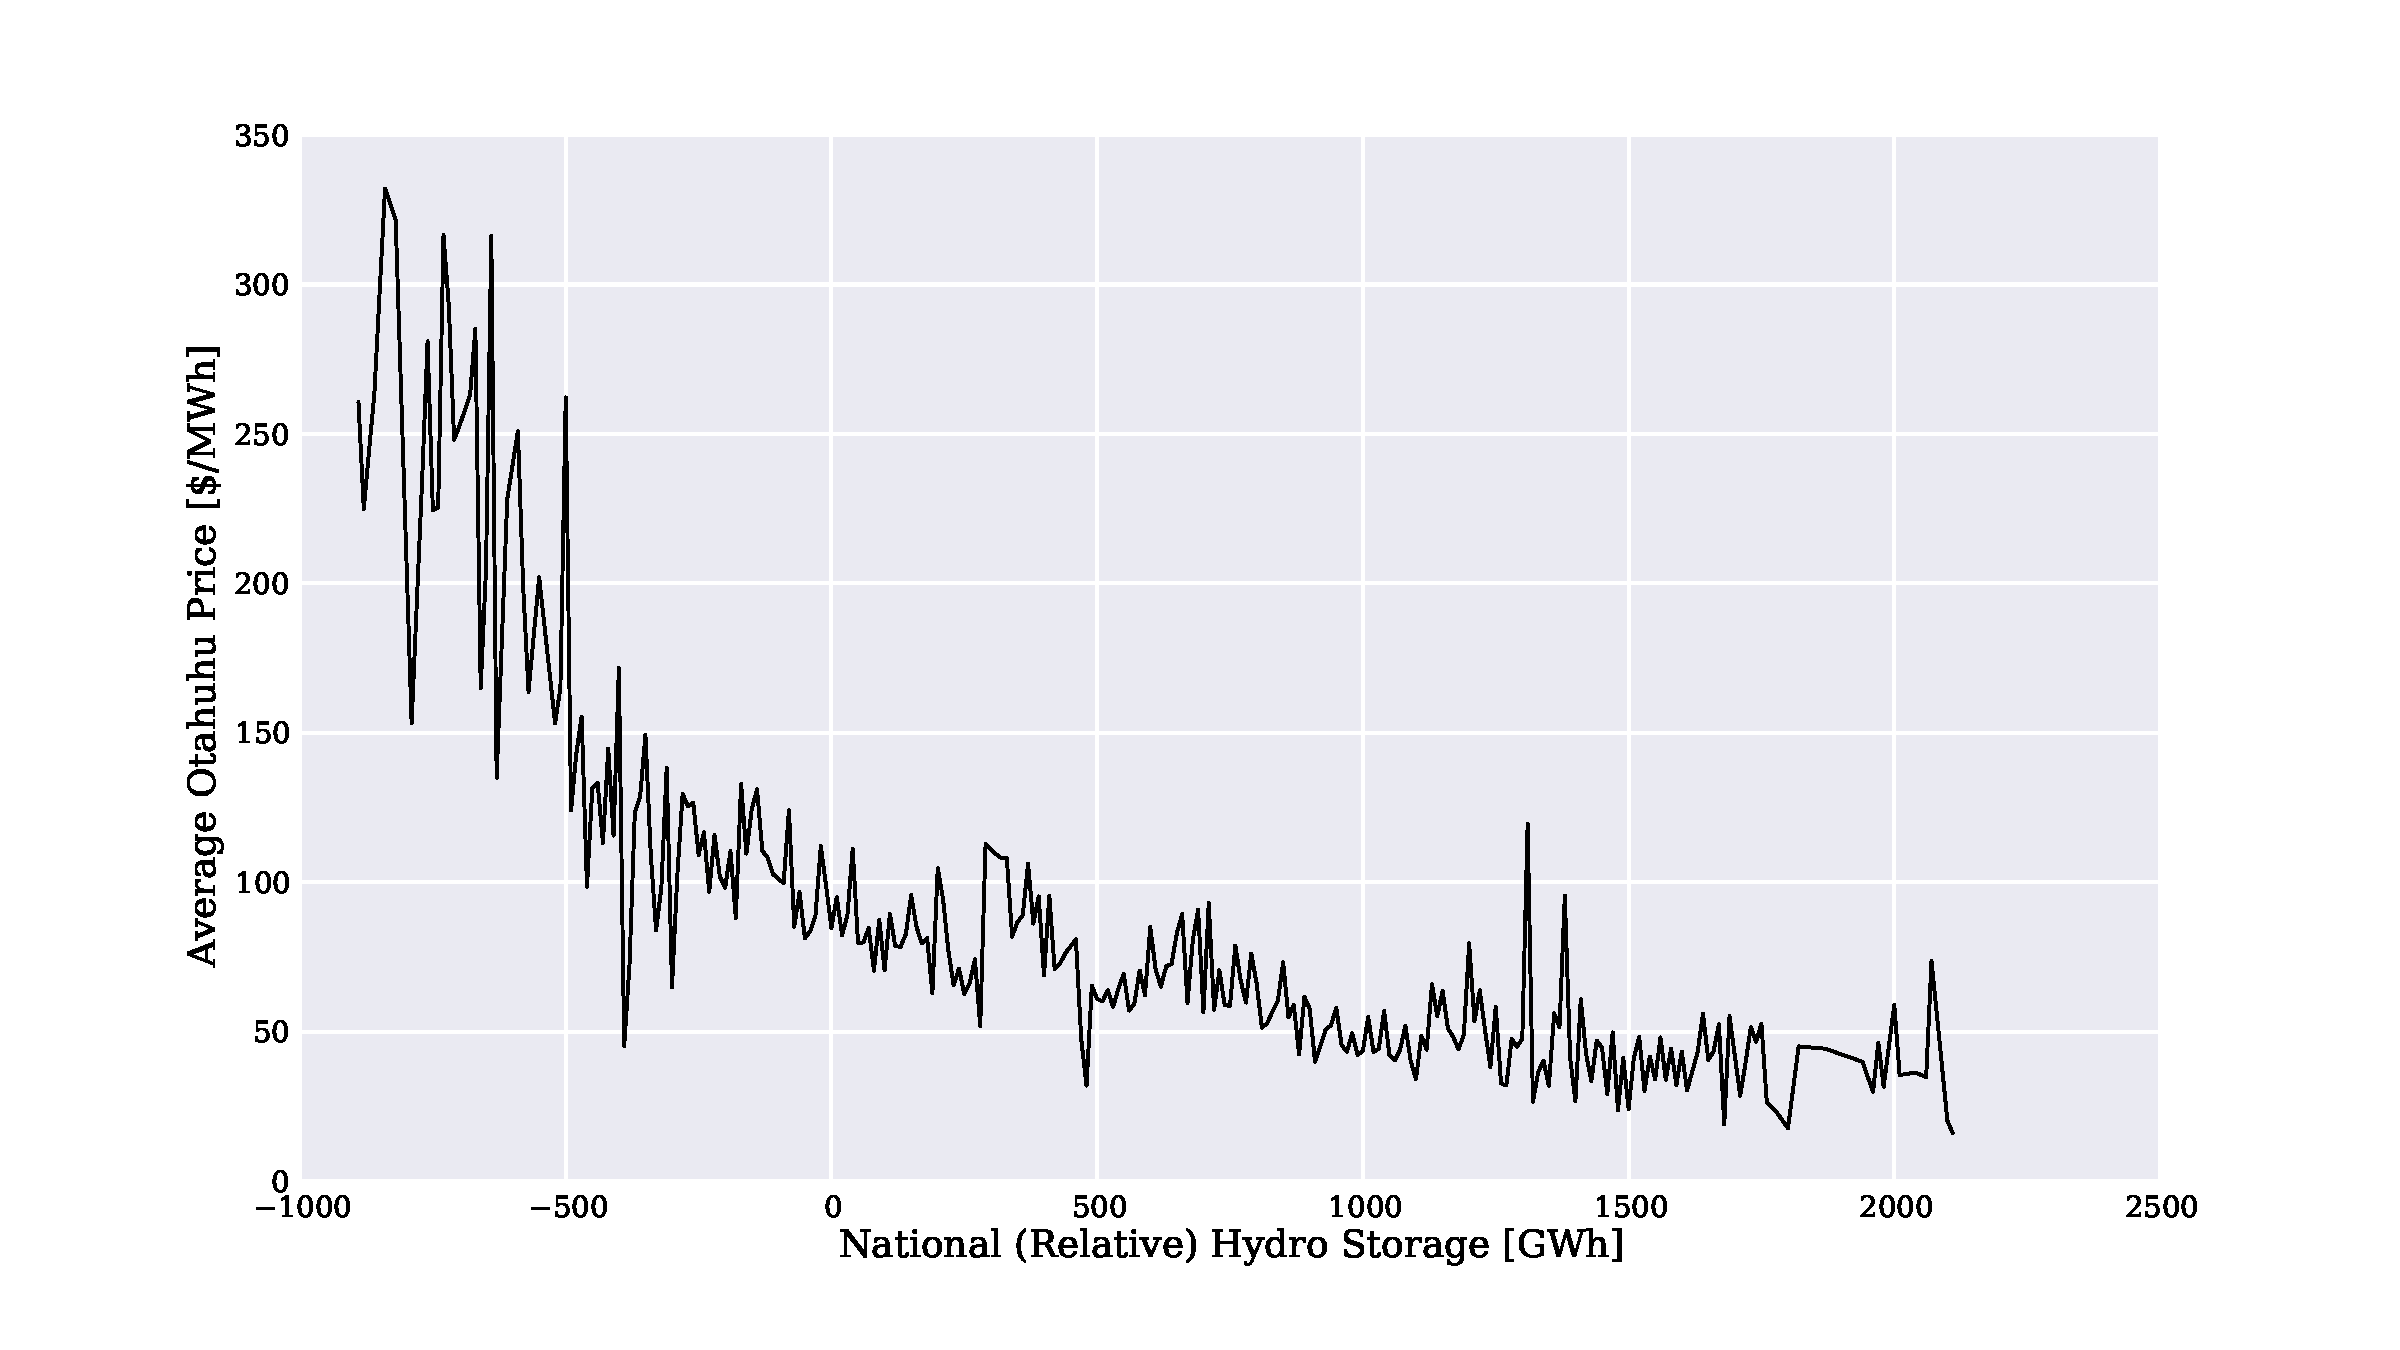
\includegraphics[width=0.95\textwidth]{img/price_and_hydrology.pdf}
\caption{As expected, the less water we have (relative to the lower decile
for the time of year) the higher the average price}
\end{figure}
\end{frame}

\begin{frame}{Average Demand at Different Price Points}
\begin{figure}
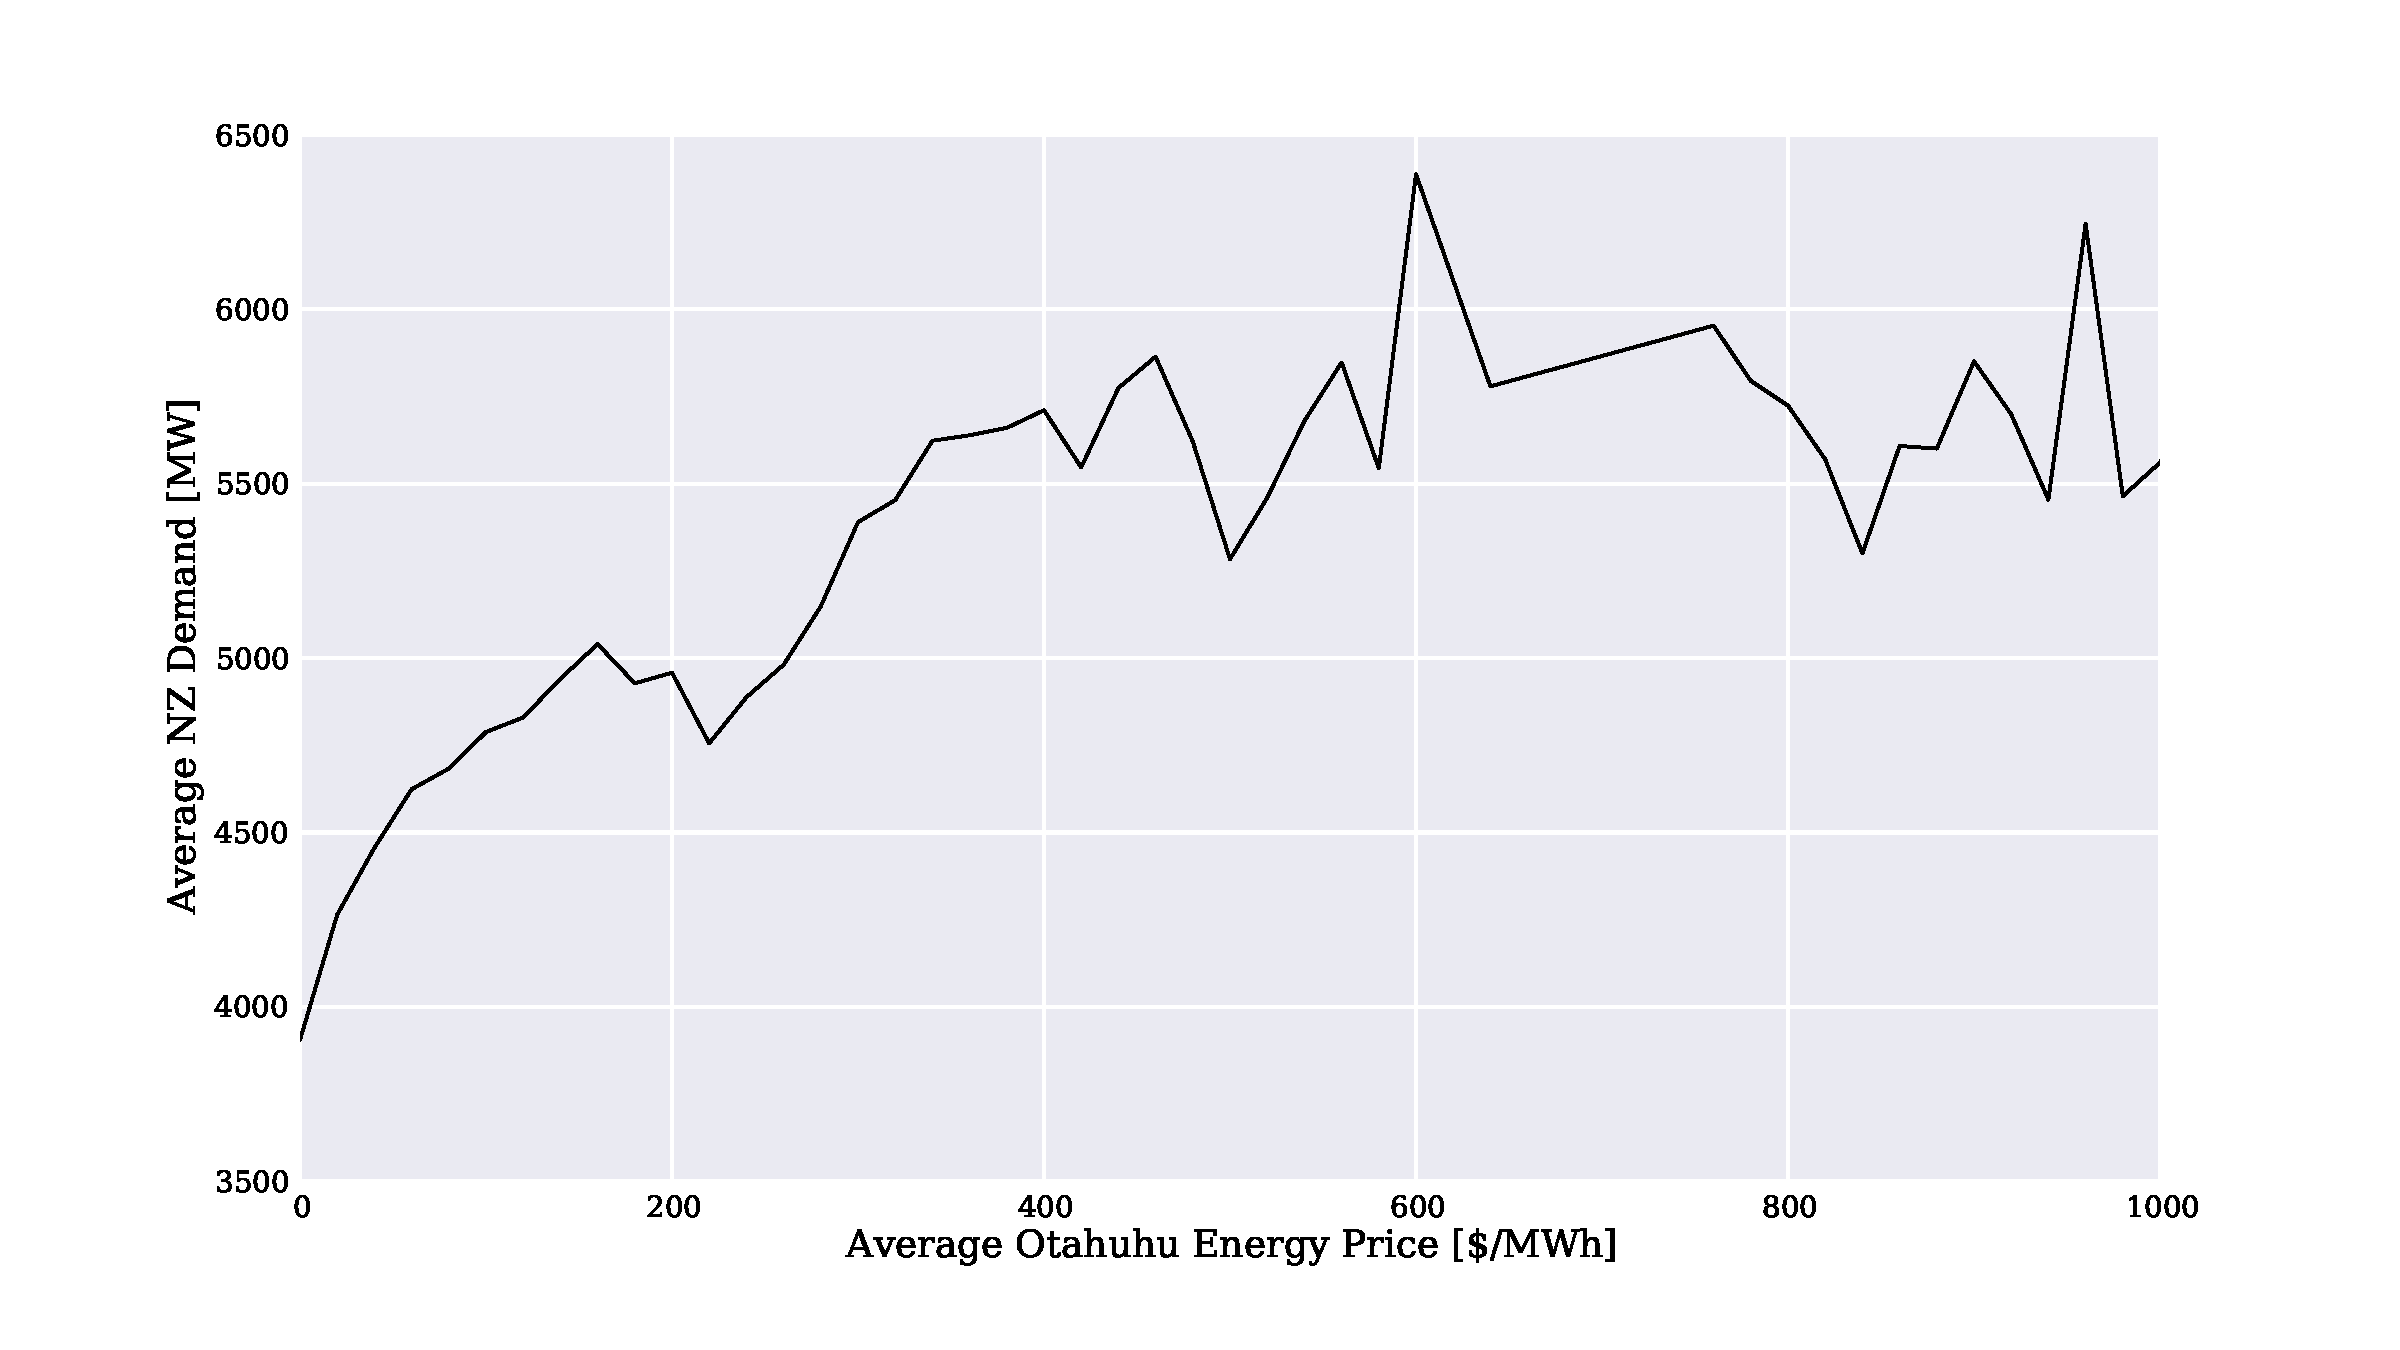
\includegraphics[width=0.95\textwidth]{img/demand_and_price.pdf}
\caption{The relationship between high demand and high prices isn't so
clear when the reverse situation occurs}
\end{figure}
\end{frame}

\begin{frame}{Average Hydrology at Different Price Points}
\begin{figure}
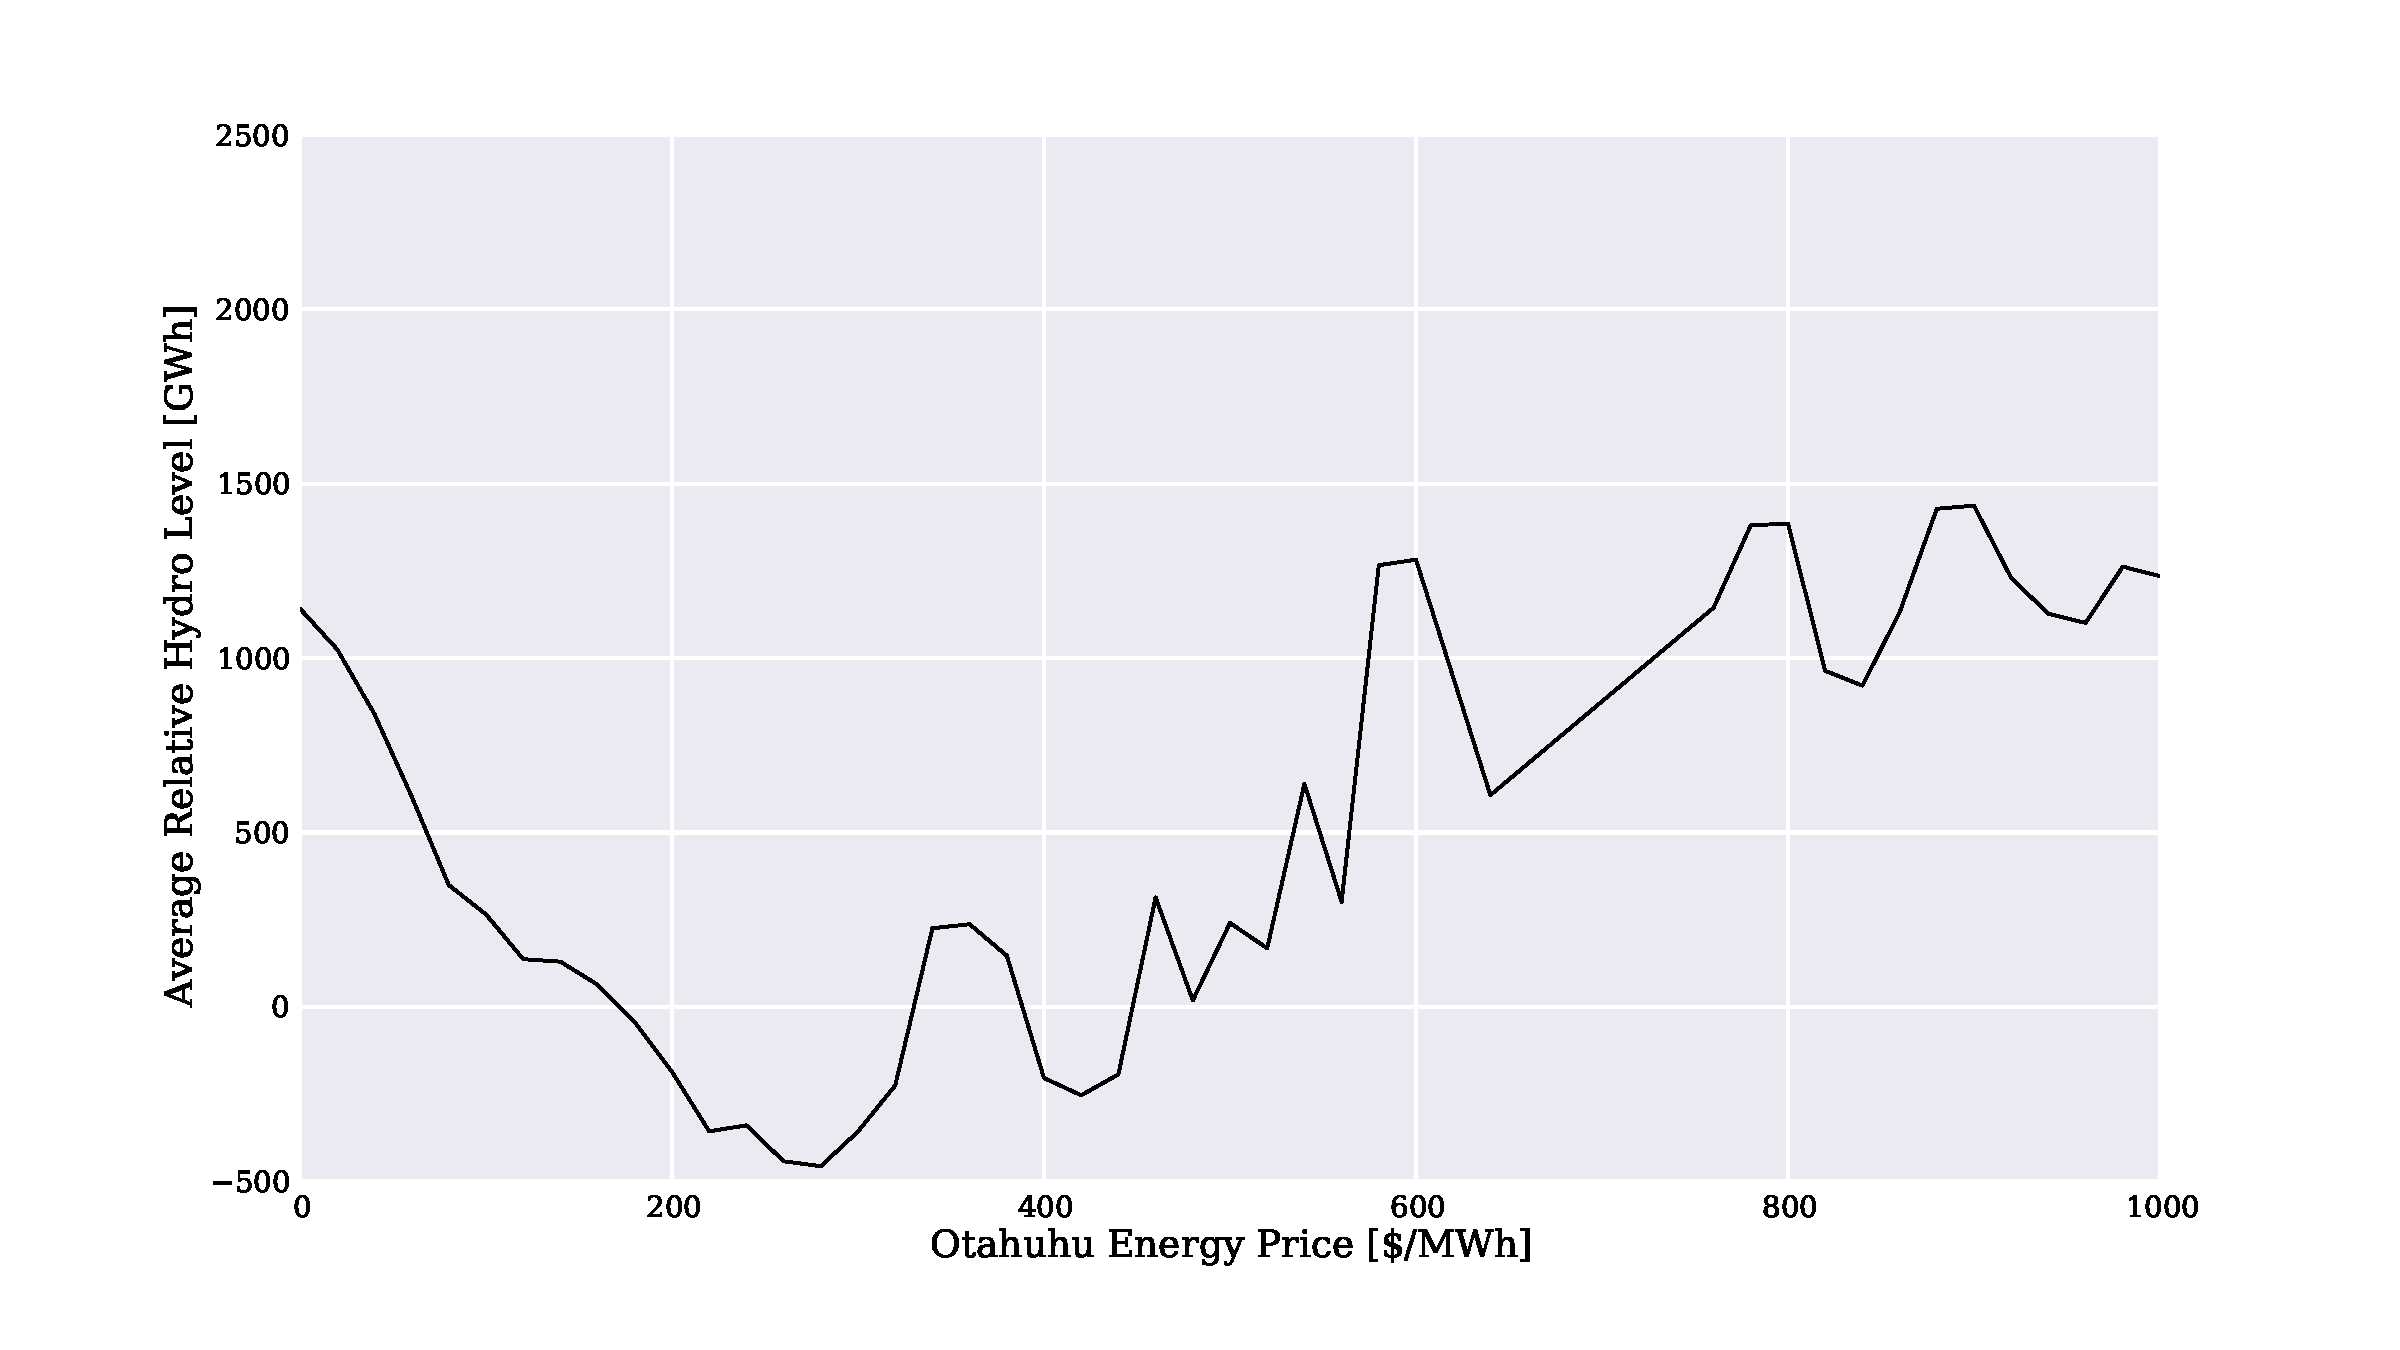
\includegraphics[width=0.95\textwidth]{img/hydrology_and_price.pdf}
\caption{The Paradox of Hydrology, the highest price trading periods are
associated with large quantities of water}
\end{figure}
\end{frame}

\begin{frame}{Constraints at different price levels}
\begin{figure}
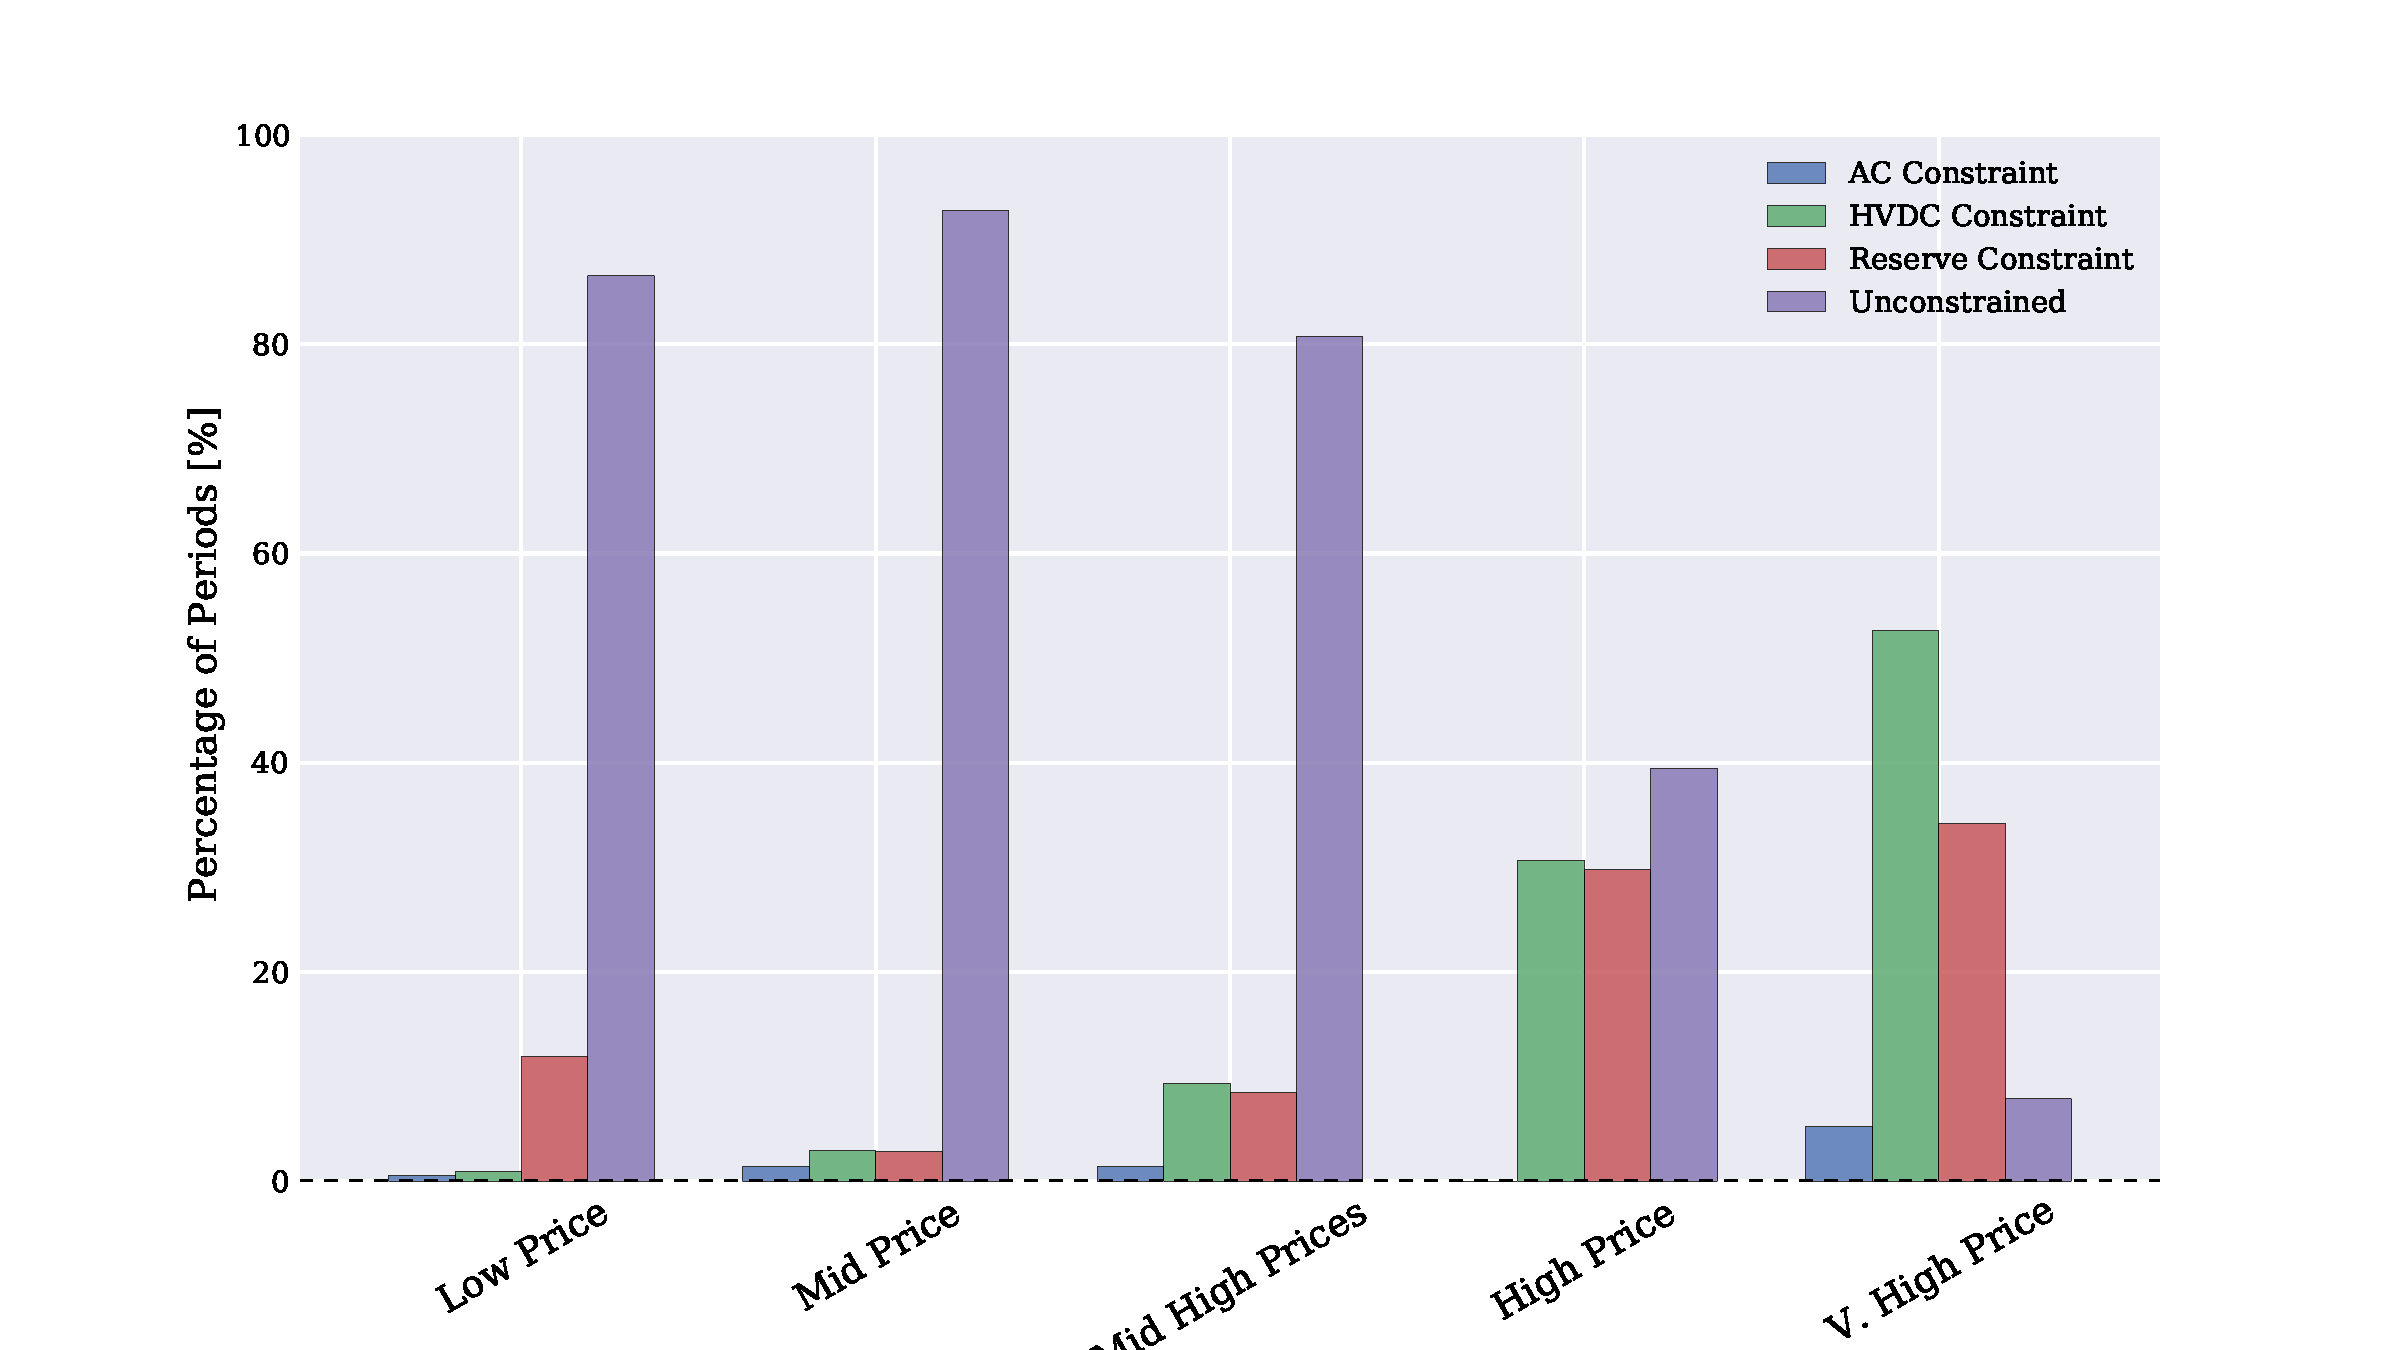
\includegraphics[width=0.95\textwidth]{img/constrained_periods_analysis.pdf}
\caption{Aggregate assessment of constraints in the New Zealand Market}
\end{figure}
\end{frame}

\begin{frame}{Specific Constraints}
\begin{table}
\caption{Constraints binding during the top 155 priced trading periods}
\begin{tabular}{lrrrr}
\toprule
{} &  Occurences &  Mean &  Min &  Max \\
\midrule
Waikato Block SIR Constraint &          41 &   768 &    0 & 4948 \\
Waikato Block FIR Constraint &          40 &   491 &    2 & 3834 \\
Tokaanu SIR Constraint       &          26 &   417 &    2 & 1010 \\
Waikato Block Dispatch       &          21 &  1409 &   13 & 4653 \\
Tokaanu FIR Constraint       &          13 &  1009 &    0 & 4409 \\
\bottomrule
\end{tabular}
\end{table}
\end{frame}

\begin{frame}{Contextualising the Constraints}
\centering
\begin{figure}
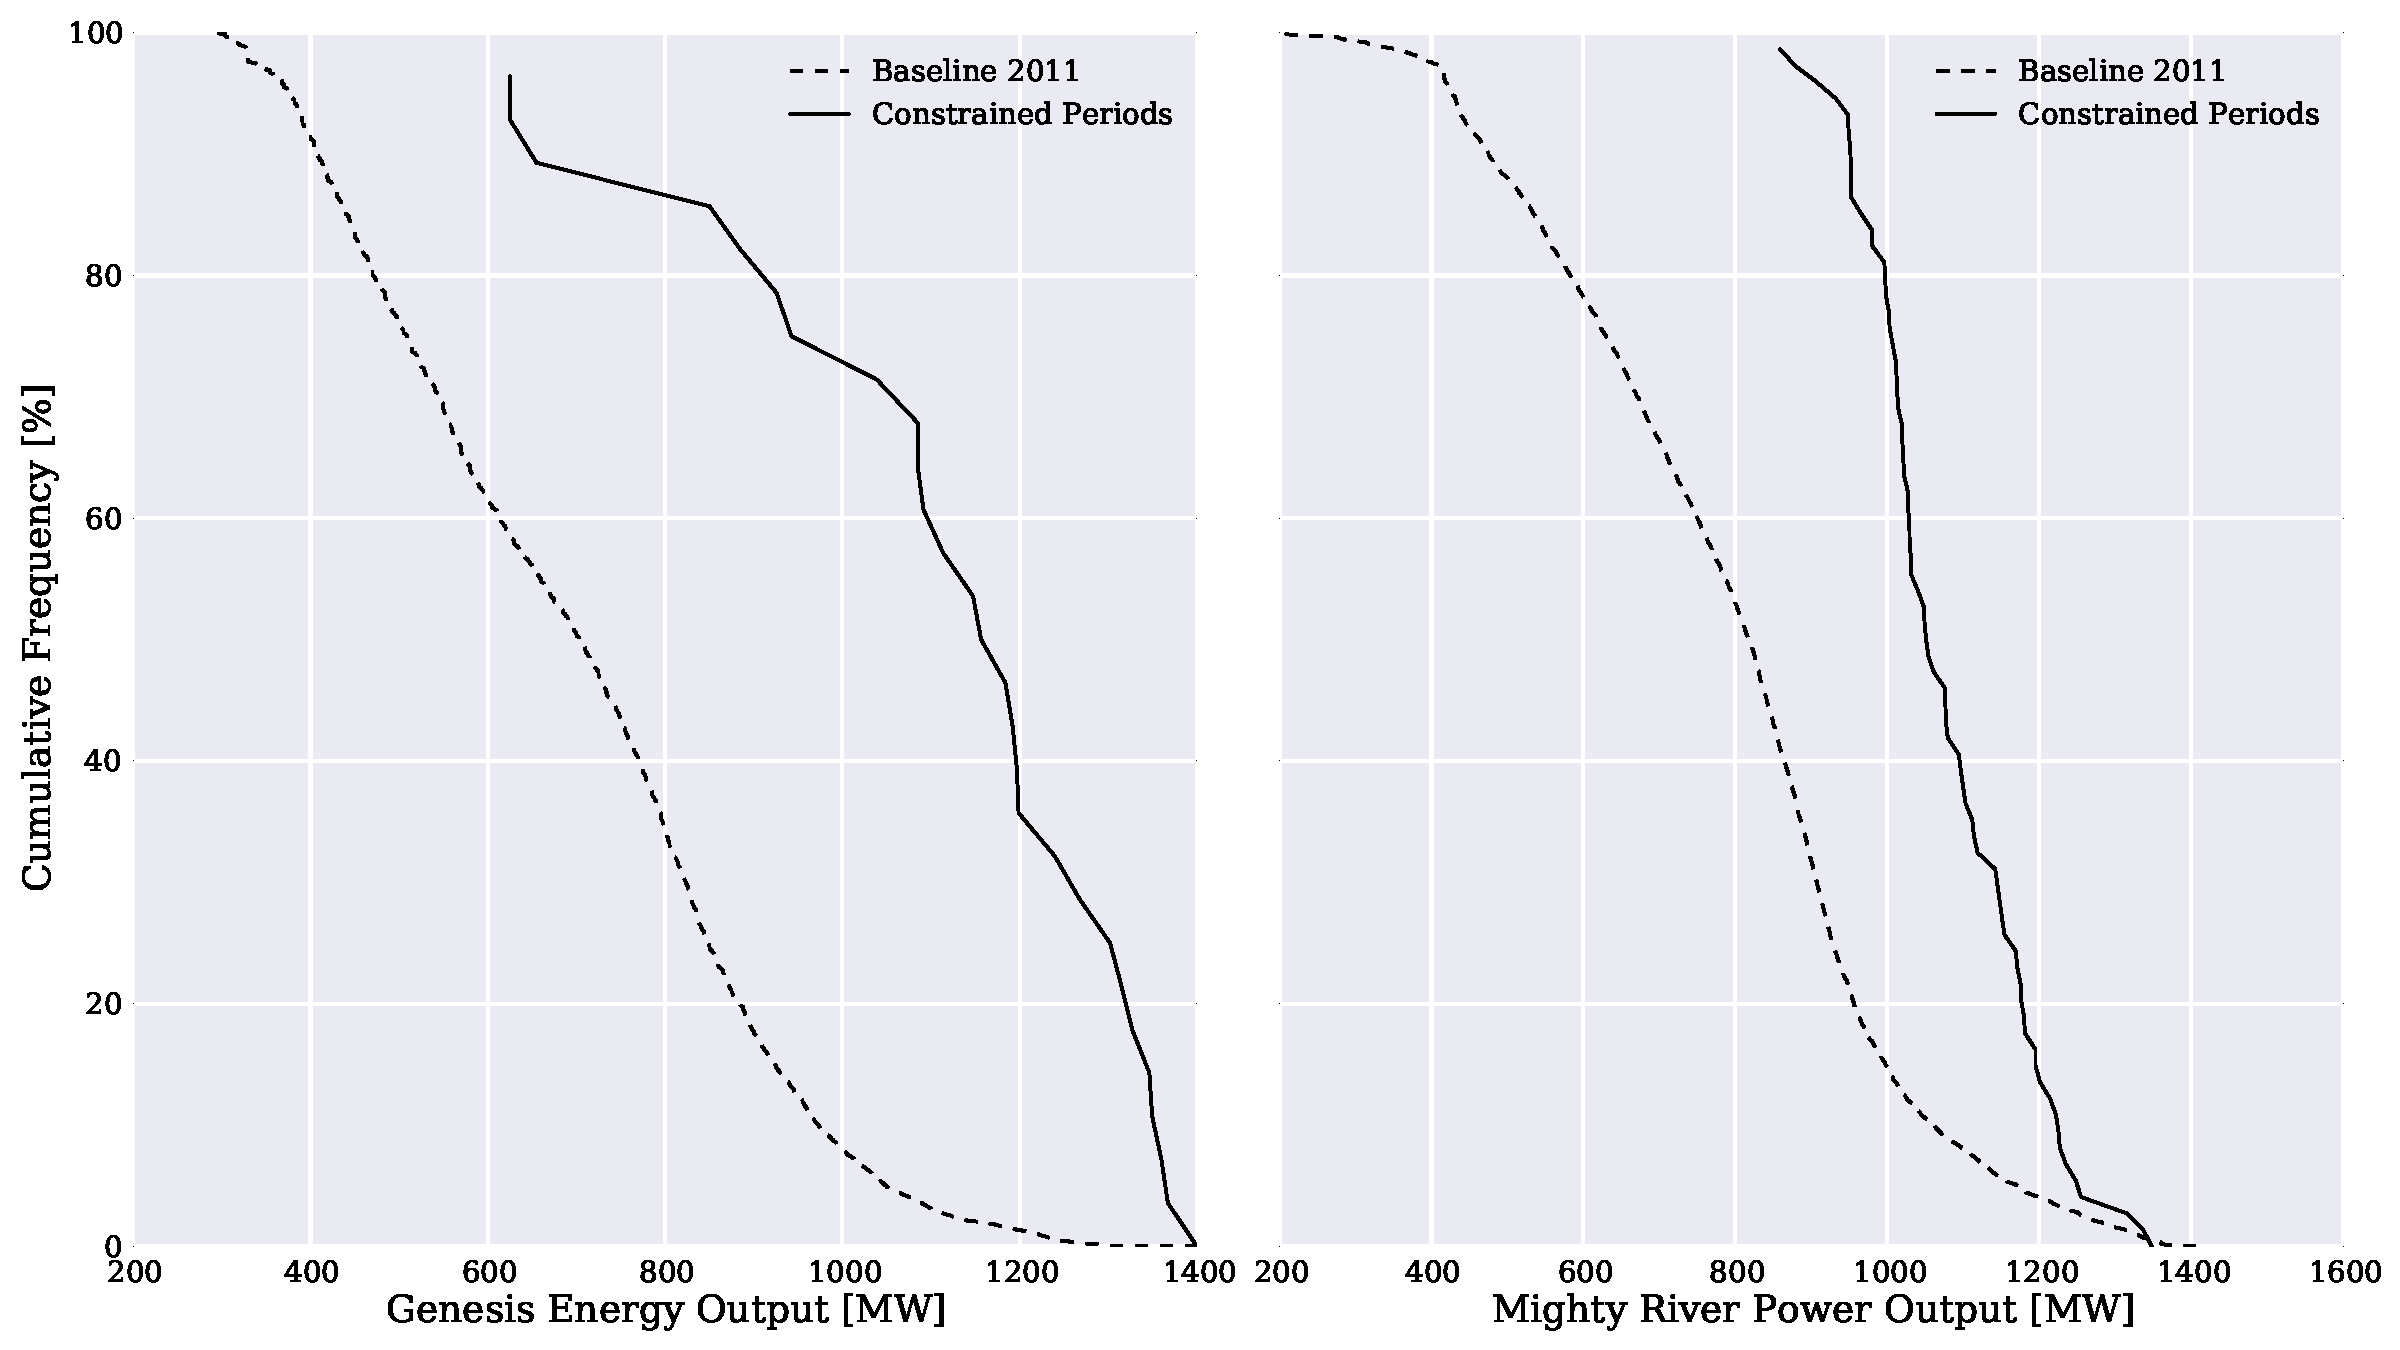
\includegraphics[width=0.95\textwidth]{img/gen_mrp_output_vs_baseline.pdf}
\caption{Dispatch (CDF) of Genesis and Mighty River during Constraints Periods
(Genesis for Tokaanu Constraints, Mighty River for Waikato Constraints)
compared with the overall CDF for the providers}
\end{figure}
\end{frame}

\section{\scshape Equilibrium Models}
\begin{frame}
\vspace{1.5cm}
\begin{center}
{\Huge\textit{Equilibrium Models}}
\end{center}
\end{frame}

\begin{frame}{Overview}
\begin{itemize}
\item Equilibrium Models give insight into how providers will act under
simplified assumptions.
\item Often used in market power assessments (e.g. UK/USA)
\item Integrating Reserve Markets is difficult
\item Some Prior art, but not as relevant to NZ.
\item Use Linear Supply Functions
\end{itemize}
\end{frame}

\begin{frame}{Generator Problem}
\begin{eqnarray*}
C(g_{n,i}) &=& (\beta_{n,i} + 0.5\gamma_{n,i}g_{n,i})g_{n,i} \\
C(r_{n,i}) &=& \alpha_{n,i}r_{n,i} \\
R(c) &=& \sum_{n,i} \lambda_{n}g_{n,i} + \sum_{n,i} \mu_{n}r_{n,i} \\
\pi(c) &=& \sum_{n,i} (\lambda_{n} - \beta_{n,i} - \gamma_{n,i}g_{n,i})g_{n,i} + \sum_{n,i} (\mu_{n} - \alpha_{n,i})r_{n,i}
\end{eqnarray*}
\end{frame}

\begin{frame}{Setting up the Equilibrium}
\begin{itemize}
\item Want to Maximise Profit
\item Generator specifically takes into account how they influence the others
\item Introduce a Leader - Follower problem
\item ISO acts as a Follower
\item Introduce KKT conditions as constraints to the Generator Problem
\end{itemize}
\end{frame}

\begin{frame}{ISO Primal Problem}
\begin{eqnarray*}
\min & \sum_{n,i} (\beta^{*}_{n,i} + 0.5\gamma^{*}_{n,i}g_{n,i})g_{n,i} + \sum_{n,i} \alpha^{*}_{n,i}r_{n,i} & \\
\text{st} & \sum_{i \in n(i)} g_{n,i} + \sigma_{n}f = d_{n} \hspace{0.2cm} & \forall n \\
& \sum_{i \in n(i)} r_{n,i} -\sigma_{n}f \ge 0 \hspace{0.2cm} & \forall n \\
& 0 \le g_{n,i} \le G_{n,i} & \forall n, i \\
& 0 \le r_{n,i} \le R_{n,i} & \forall n, i
\end{eqnarray*}
\end{frame}

\begin{frame}{ISO Dual Problem}
\begin{eqnarray*}
\max &\sum_{n} d_{n}\lambda_{n} - \sum_{n,i} 0.5\gamma^{*}_{n,i}g_{n,i}^{2} & \\
\mathrm{st} & \lambda_{n} \le \beta^{*}_{n,i} + \gamma^{*}_{n,i}g_{n,i} & \forall n, i \\
& \mu_{n} \le \alpha^{*}_{n,i} & \forall n, i \\
& \sum_{n} \sigma_{n}(\lambda_{n} - \mu_{n}) = 0 & \forall n
\end{eqnarray*}
\end{frame}

\begin{frame}{ISO Complimentarity Conditions}
\begin{eqnarray*}
g_{n,i}(\beta^{*}_{n,i} + \gamma^{*}_{n,i}g_{n,i} - \lambda_{n}) = 0 & \forall n,i \\
r_{n,i}(\alpha^{*}_{n,i} - \mu_{n}) = 0 & \forall n, i \\
\mu_{n}(\sum_{i \in n(i)} r_{n,i} - \sigma_{n}f) = 0 & \forall n
\end{eqnarray*}
\end{frame}

\begin{frame}{Full Problem Definition}
\begin{eqnarray*}
\max & \sum_{n,i} (\lambda_{n} - \beta_{n,i} - 0.5\gamma_{n,i}g_{n,i})g_{n,i}  & \\
& \qquad + \sum_{n,i} (\mu_{n} - \alpha_{n,i})r_{n,i} & \\
\mathrm{st} &\sum_{i \in n(i)} g_{n,i} + \sigma_{n}f = d_{n} \hspace{0.2cm} & \forall n \\
&\sum_{i \in n(i)} r_{n,i} -\sigma_{n}f \ge 0 \hspace{0.2cm} & \forall n \\
& 0 \le g_{n,i} \le G_{n,i} & \forall n, i \\
& 0 \le r_{n,i} \le R_{n,i} & \forall n, i \\
& \lambda_{n} \le \beta^{*}_{n,i} + \gamma^{*}_{n,i}g_{n,i} & \forall n, i \\
& \mu_{n} \le \alpha^{*}_{n,i} & \forall n, i \\
& \sum_{n} \sigma_{n}(\lambda_{n} - \mu_{n}) = 0 & \forall n \\
& g_{n,i}(\beta^{*}_{n,i} + \gamma^{*}_{n,i}g_{n,i} - \lambda_{n}) = 0 & \forall n,i \\
& r_{n,i}(\alpha^{*}_{n,i} - \mu_{n}) = 0 & \forall n, i \\
& \mu_{n}(\sum_{i \in n(i)} r_{n,i} - \sigma_{n}f) = 0 & \forall n
\end{eqnarray*}
\end{frame}

\begin{frame}{Why would I do this}
\begin{itemize}
\item I'm a Masochist?
\item Theoretical Insights can lead to interesting conclusions
\item Help explain the why, not just the what
\item Publishable
\end{itemize}
\end{frame}

\begin{frame}{Preliminary Results}
\begin{itemize}
\item ``Blocking'' behavior has been observed
\item When blocked the other participant will seek to equalise prices.
\item Pre HVDC upgrade Meridian self withholding to not induce HVDC reserve constraints
\item ``Optimal'' was most likely for them to generate 200-300 MW more at times
\item Increase in MW leads to a decrease in price at your node, self defeating
\item How much do you care about the efficient use of water
\end{itemize}
\end{frame}

\section{\scshape Visualising Energy and Reserve Offers}
\begin{frame}
\vspace{1.5cm}
\begin{center}
{\Huge\textit{Visualising Energy and Reserve Offers}}
\end{center}
\end{frame}

\begin{frame}{Understanding Tradeoffs}
\begin{itemize}
\item Reserve and Energy are linked
\item Unit Capability
\item Energy Price
\item Reserve Price
\item Security Constraints can be very important
\end{itemize}
\end{frame}

\begin{frame}{The Inverse Bathtub}
\begin{figure}
\centering
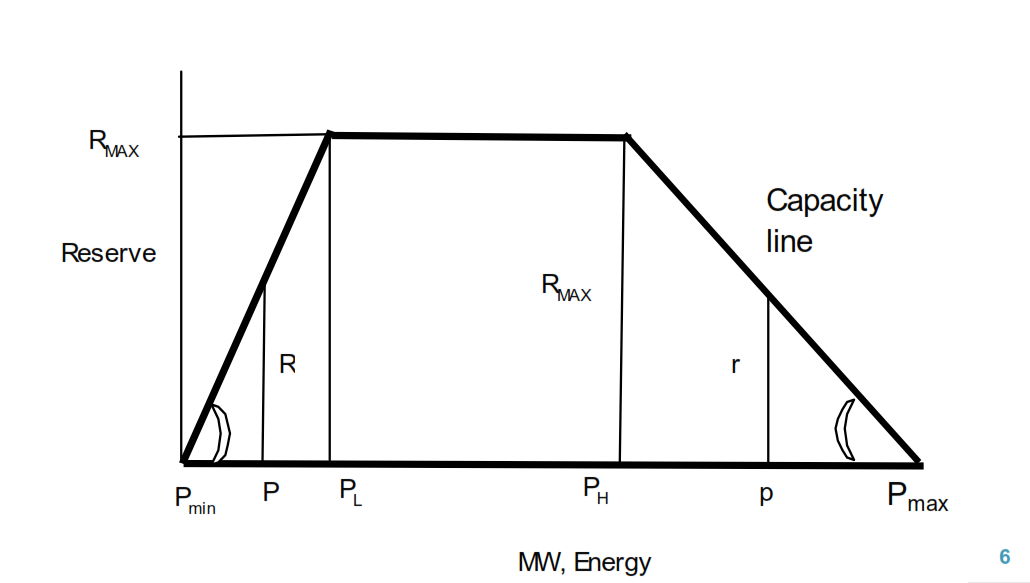
\includegraphics[width=0.95\textwidth]{img/Bathtub_Constraint_Image.png}
\caption{Depiction of the technical constraints limiting energy and reserve
offers, proportionality, capacity, unit capability constraints, Bhujanga
Chakrabarti, System Operator}
\end{figure}
\end{frame}

\begin{frame}{Flaws with the representation}
\begin{itemize}
\item Technically Feasible does not imply Economically Feasible
\item No consideration of price
\item Single Unit Representation
\end{itemize}
\center{{\scshape Improving the Representation}}
\begin{itemize}
\item Energy Prices and Reserve Prices are important
\item Combinations are importants
\end{itemize}
\end{frame}

\begin{frame}{Single Unit}
\begin{figure}
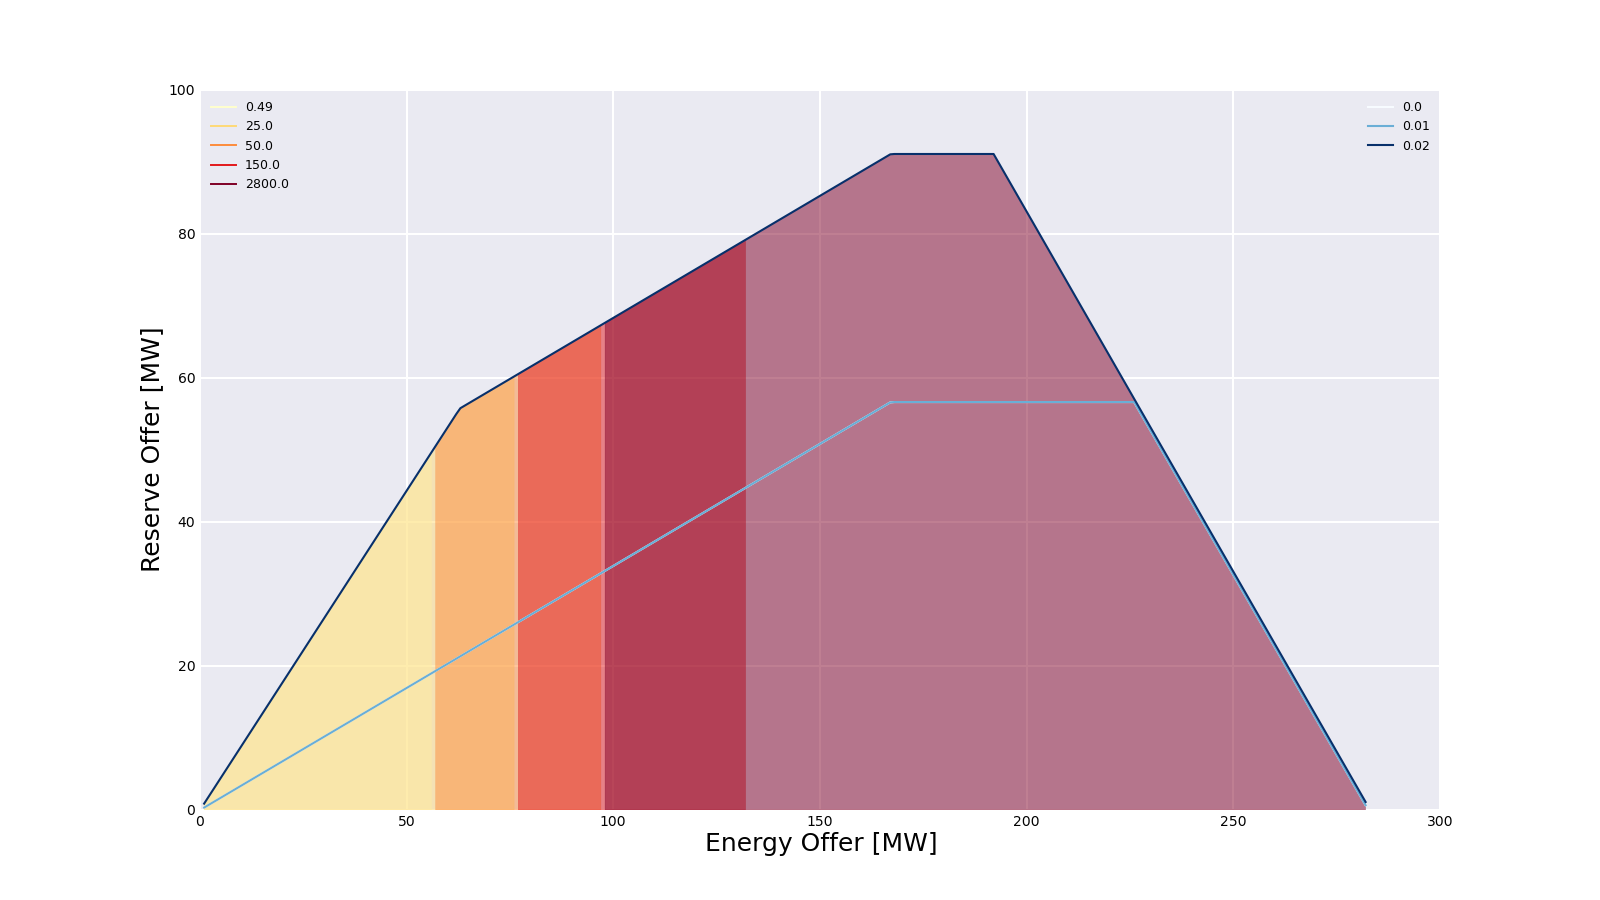
\includegraphics[width=0.95\textwidth]{img/mti_station_fan.png}
\caption{Representation of the Fan Offered for Maraetai for TP19}
\end{figure}
\end{frame}

\begin{frame}{Single Company}
\begin{figure}
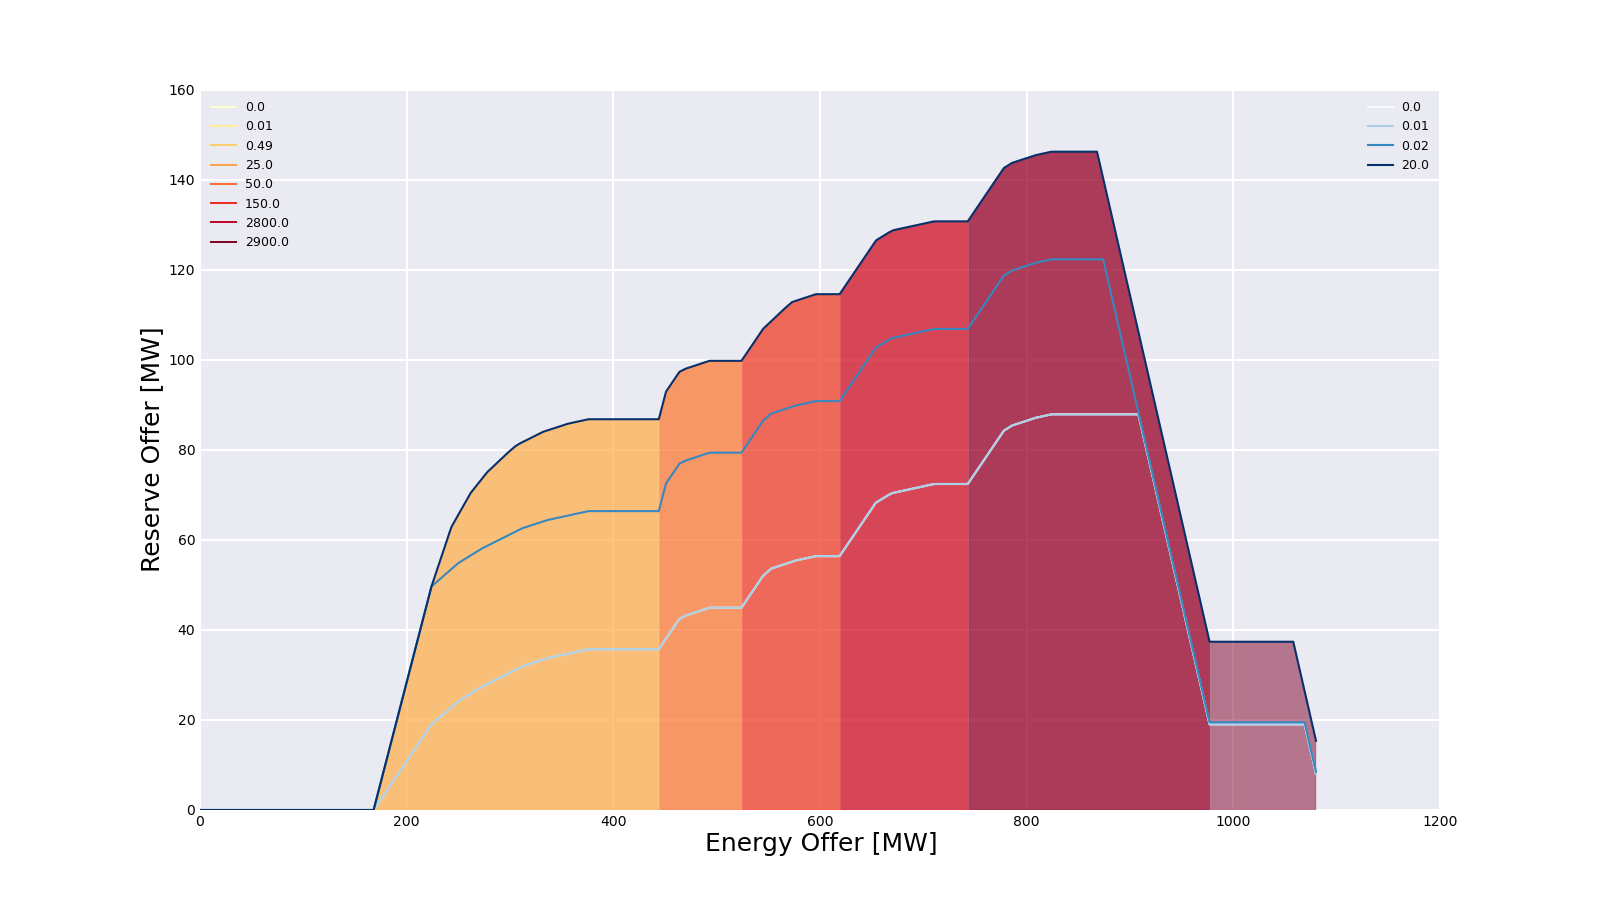
\includegraphics[width=0.95\textwidth]{img/mrpl_fan_curve.png}
\caption{Representation of the Fan offers by Mighty River Power for TP19}
\end{figure}
\end{frame}

\begin{frame}{Entire Island}
\begin{figure}
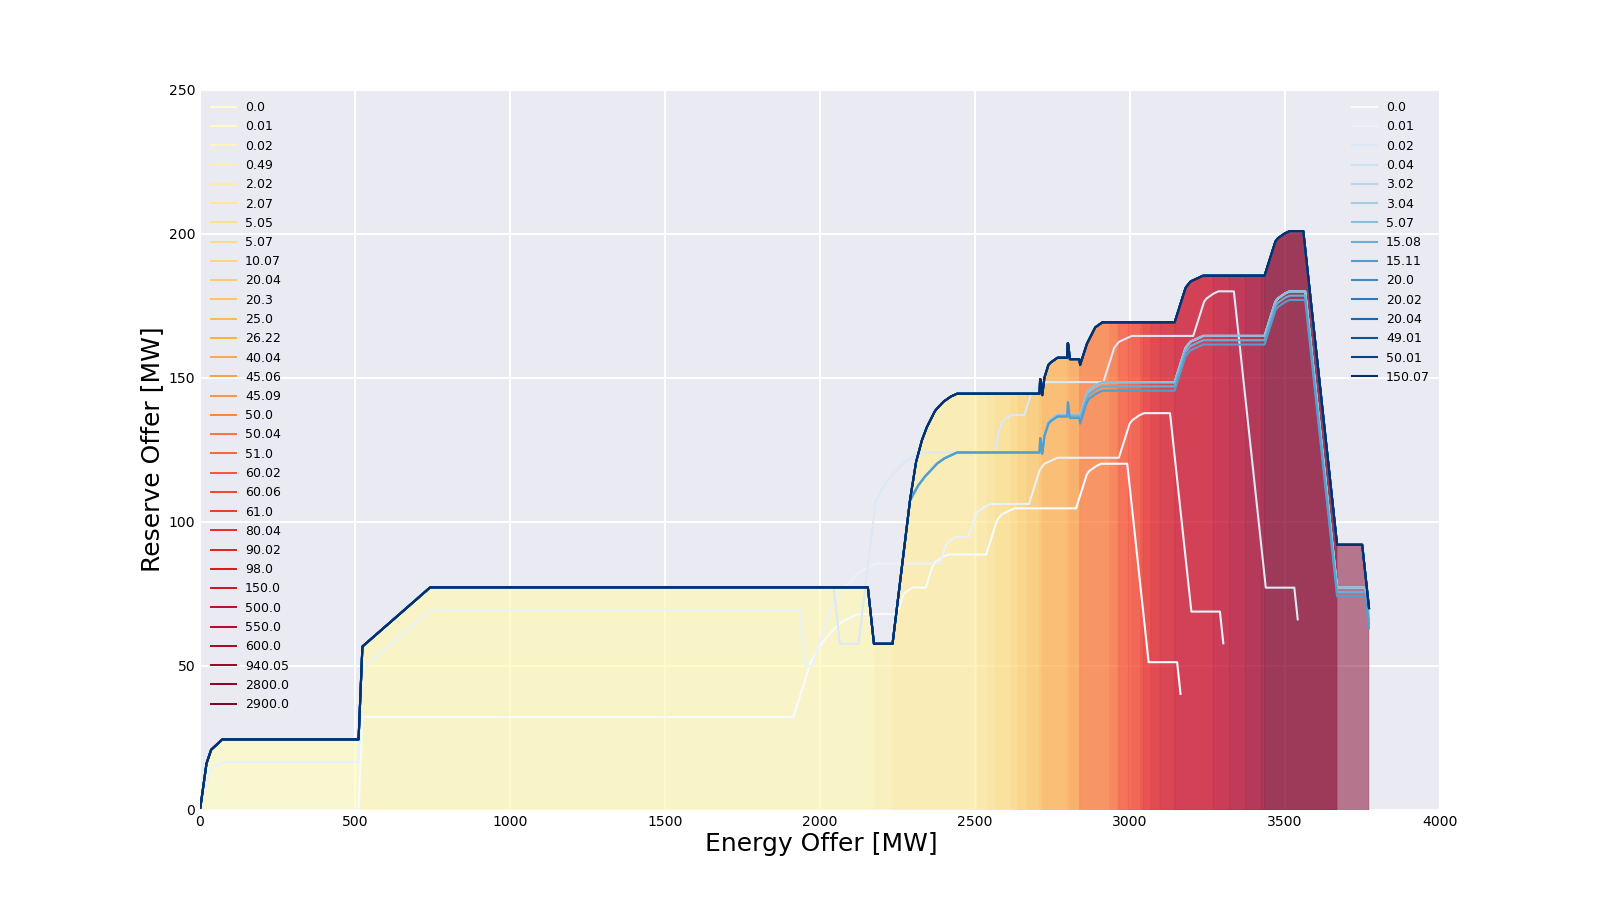
\includegraphics[width=0.95\textwidth]{img/full_ni_fan.png}
\caption{Full Representation of the North Island Offer Fan for TP19}
\end{figure}
\end{frame}

\begin{frame}{How this works}
\begin{itemize}
\item Create an incremental capacity line for each unit of (1MW increments) linked with energy price.
\item For each reserve pairings create a corresponding incremental reserve line bound by the bathtub constraints.
\item Do a little bit of book keeping for the combined capacity constraint.
\item Produce a number of station fans which can then be filtered and grouped
based upon reserve price.
\item Create a separate ``fan'' for each reserve price and offer.
\end{itemize}
\end{frame}

\begin{frame}{How this works v2}
\begin{itemize}
\item Take a subset of the stations
\item Filter by each unique reserve price
\item Group by each unique reserve price, offer precedence to higher ratio units
\item Sort by energy price, reserve price, reserve ratio
\item Plot it (Actually it's dozens of automatically generated plots merged together)
\item Cross fingers it doesn't break
\end{itemize}
\end{frame}

\begin{frame}{Issues and Future Improvements}
\begin{itemize}
\item Interruptible Load Offers
\item Tail Water Depressed Offers
\item Overlay Energy and Reserve Clearing Quantites
\item Multiple technology types don't play well.
\end{itemize}
\end{frame}

\begin{frame}{Intended Use Cases}
\begin{itemize}
\item Instances of ``withholding'' reserve by pricing energy out
\item Useful Visualisation for market strategies
\item HVDC transfer operations (identifying feasibility)
\item Meridian Trading Optimisation Problem
\item Priority?
\end{itemize}
\end{frame}

\section{\scshape Bayesian Probability and Constraints}
\begin{frame}
\vspace{1.5cm}
\begin{center}
{\Huge\textit{Bayesian Probability and Constraints}}
\end{center}
\end{frame}

\begin{frame}{What conditions}
\Large
\begin{equation*}
P( \text{Constraint} | \text{State of the World} )
\end{equation*}
\end{frame}

% \begin{frame}{What conditions are linked to reserve constraints}
% \Large
% \begin{equation}
% P(\text{Constraint} | \text{State of the world})
% \end{equation}
% \normal
% \end{frame}

\begin{frame}{States of the World}
\begin{itemize}
\item Primary
\begin{itemize}
\item Hydrology
\item Time of Year
\item Time of Day
\end{itemize}
\item Derived
\begin{itemize}
\item Price
\item Demand
\item Availability
\end{itemize}
\end{itemize}
\end{frame}

\begin{frame}{Hydrology}
Problem: Hydrology is not evenly distributed, very chunky \\
Solution: \\
\begin{eqnarray*}
P(C | H) &=& \alpha P(C | \ge H) + (1 - \alpha) P (C | \le H) \\
\alpha &=& 1 - \dfrac{n}{N}
\end{eqnarray*}
\end{frame}

\begin{frame}{What does this look like}
\begin{figure}
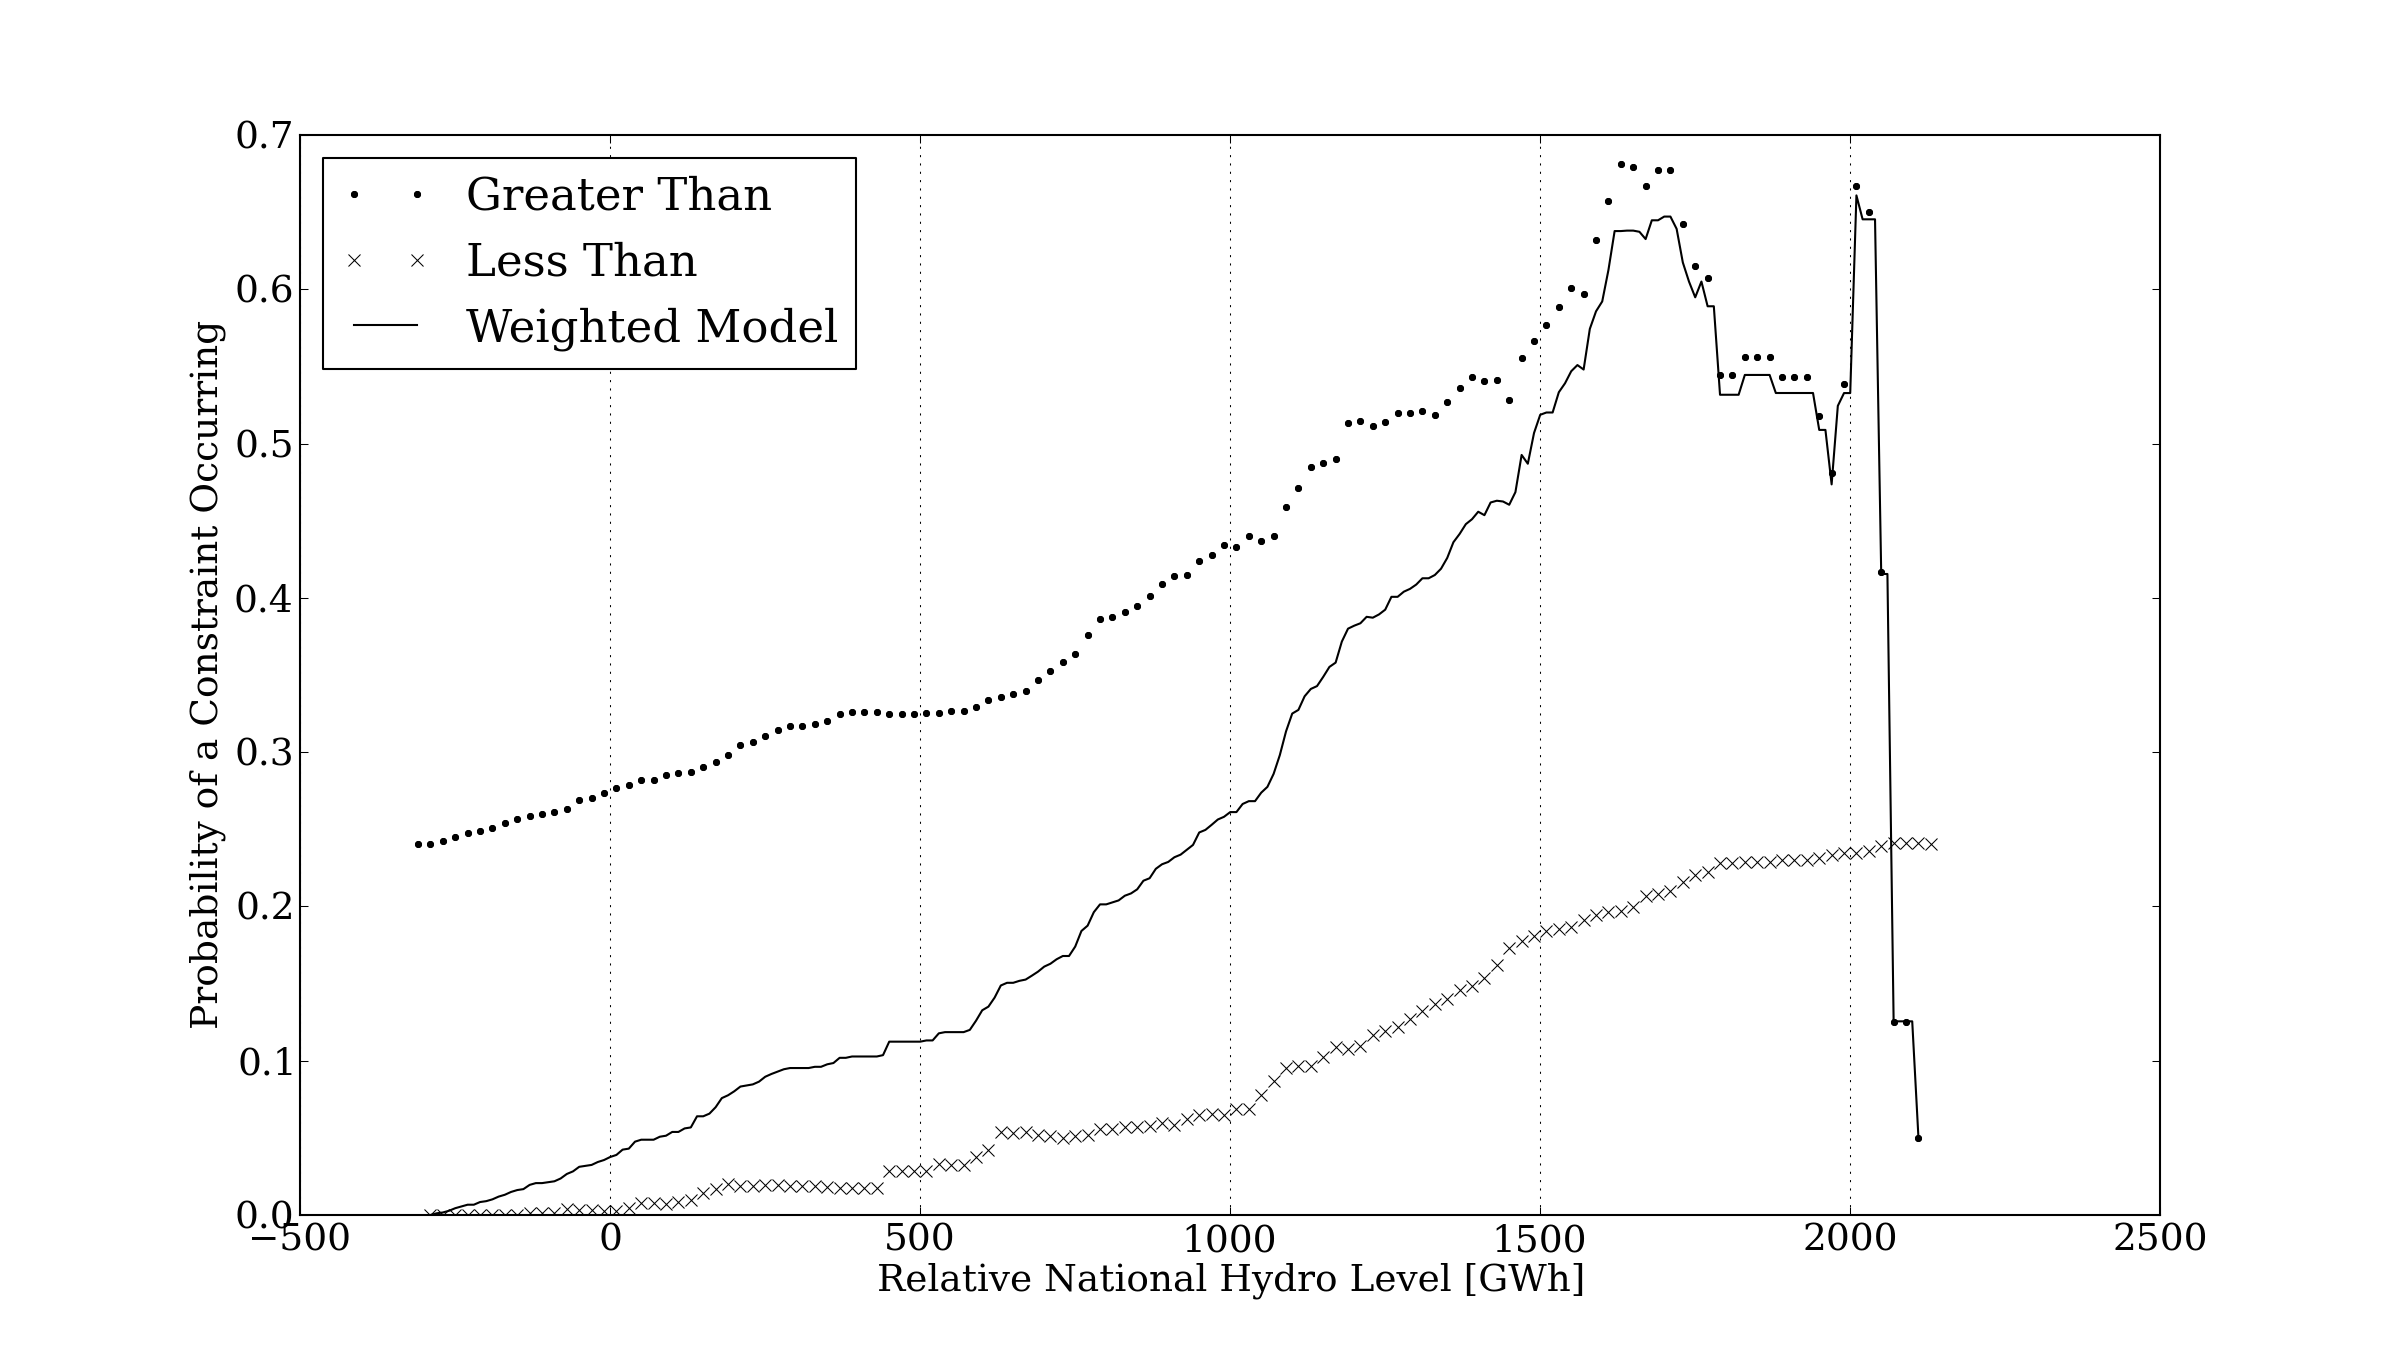
\includegraphics[width=0.95\textwidth]{img/prob_models.png}
\caption{Illustration of the weighting procedure for assessing constraints as
a function of Hydrology, time of year (Summer) and time of day (Peak)}
\end{figure}
\end{frame}

\begin{frame}{Fitting this information}
\begin{figure}
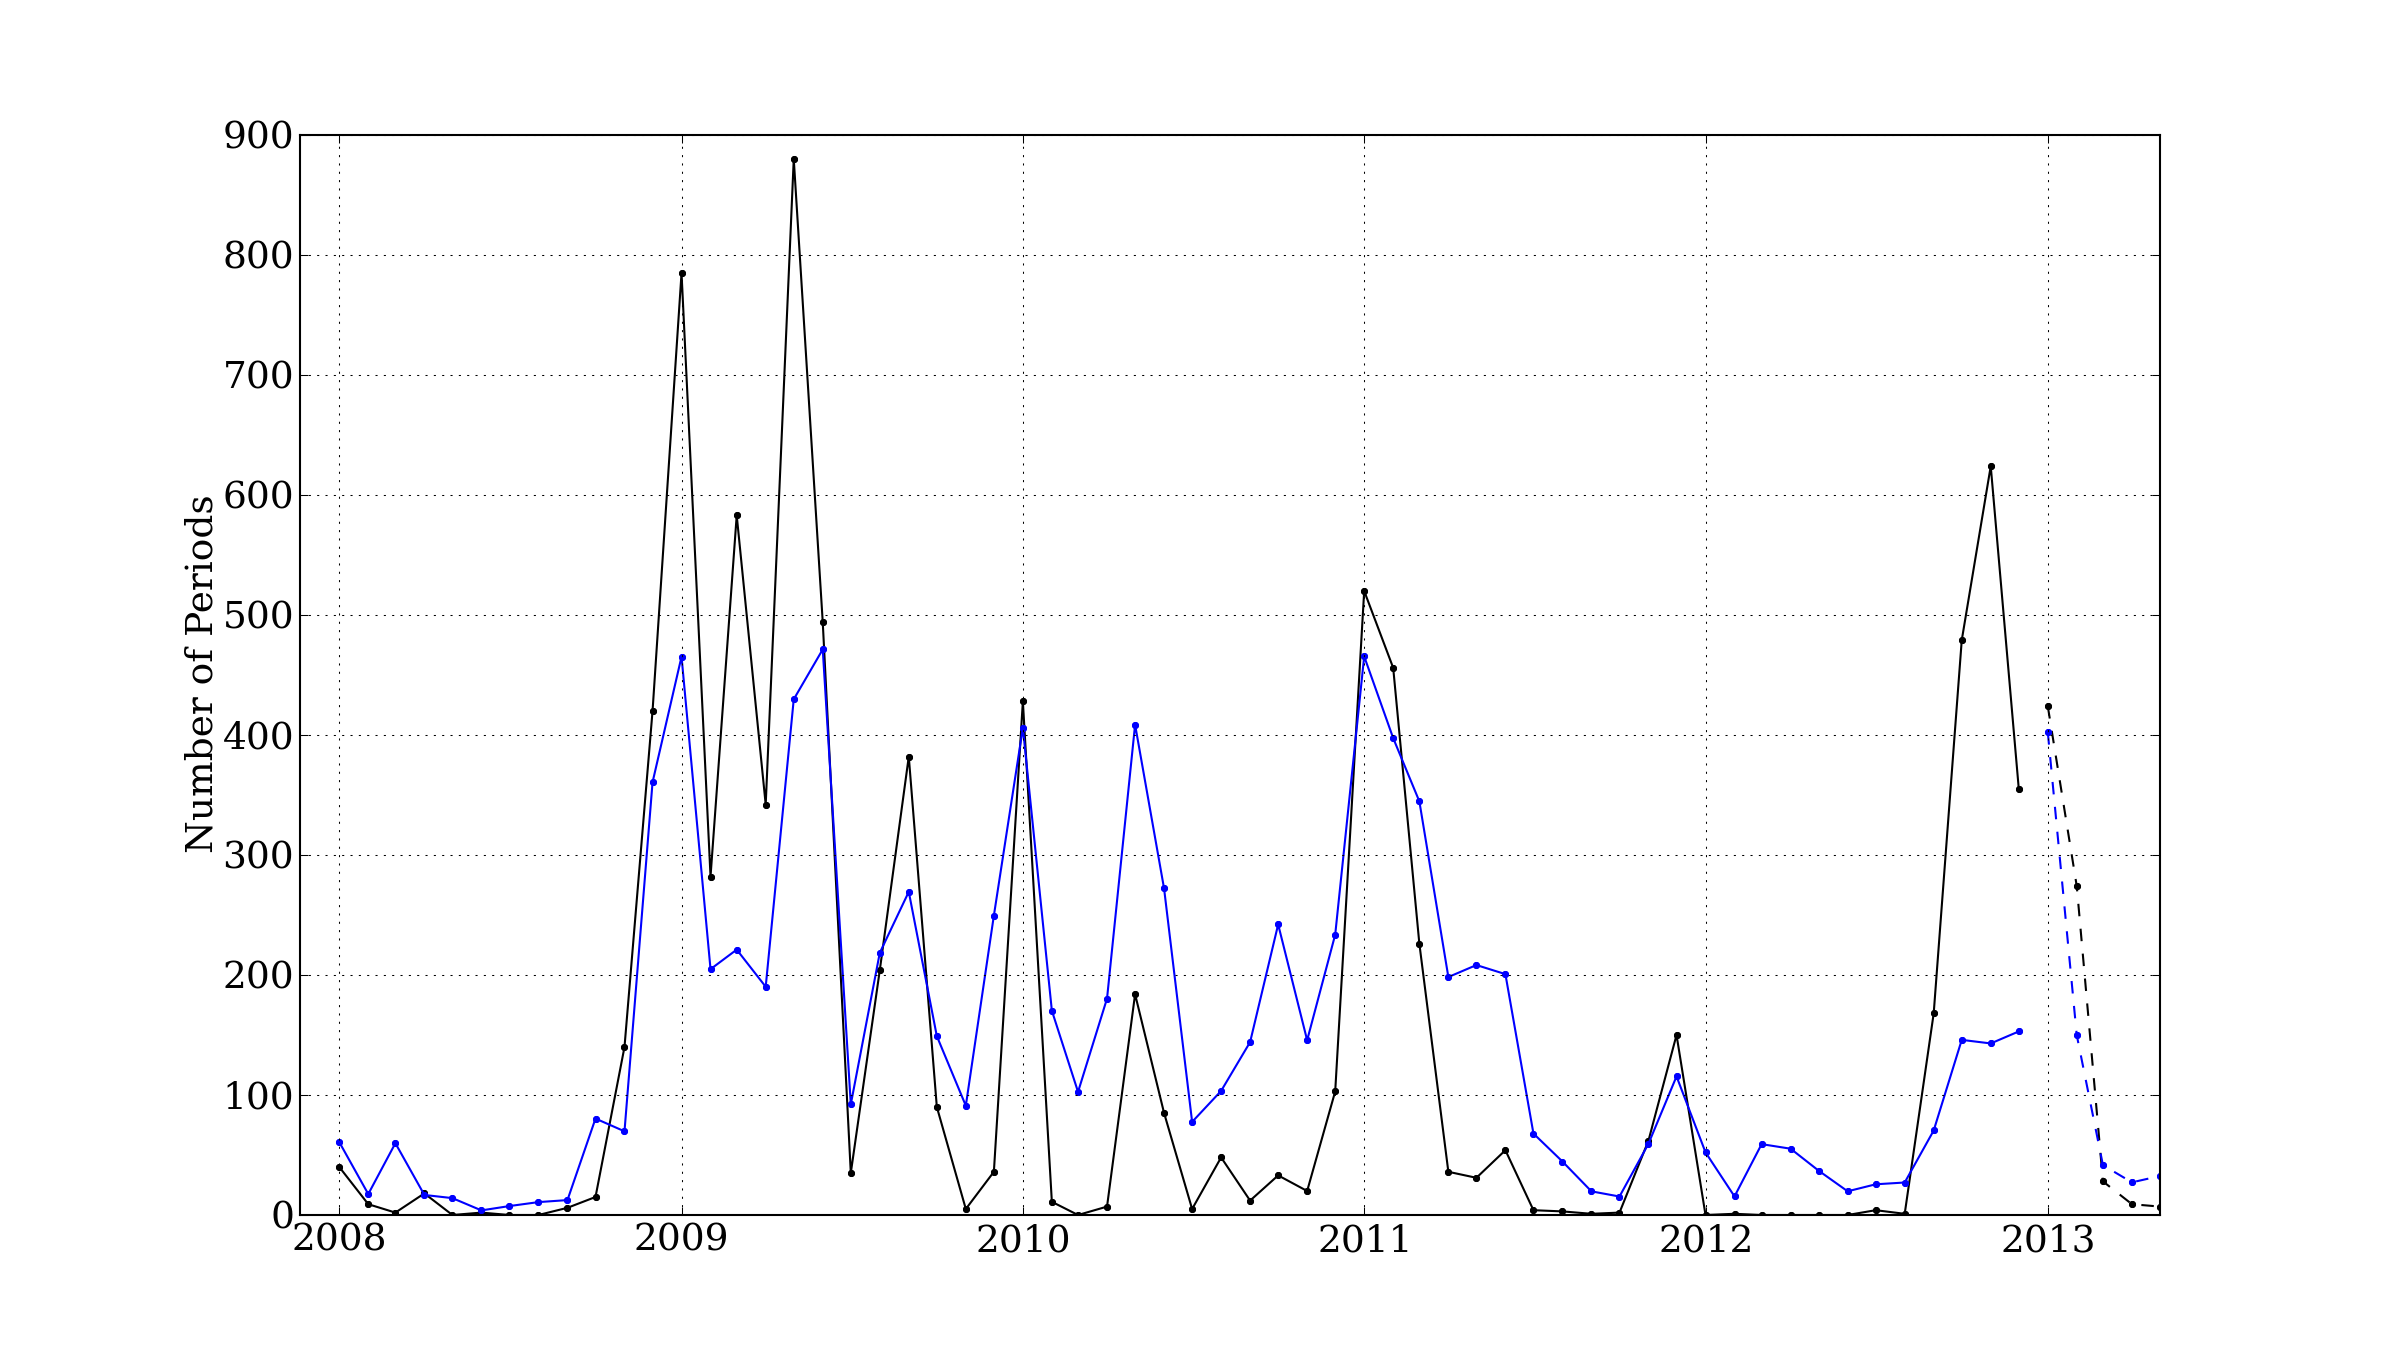
\includegraphics[width=0.95\textwidth]{img/nimodelts.png}
\caption{Fitting the model to fitted historical data (solid line) and unfitted
historical data (dashed lines).}
\end{figure}
\end{frame}

\begin{frame}{Results and Flaws}
\begin{itemize}
\item Can predict constraints in aggregate, no information about price
\item Identifies periods which are ``sensitive'' to reserve
\item Haven't had time to formalise the methodology
\item Work was done prior to HVDC commissioning
\item Appears to overweight low probability periods.
\end{itemize}
\end{frame}

\section{\scshape Open Source and Open Data}
\begin{frame}
\vspace{1.5cm}
\begin{center}
{\Huge\textit{Open Source and Open Data}}
\end{center}
\end{frame}

\begin{frame}
\vspace{1.5cm}
\begin{center}
{\Huge\textit{Why Open Source?}}
\end{center}
\end{frame}

\begin{frame}
\vspace{1.5cm}
\begin{center}
{\Huge\textit{Opaque Analysis and Trust\\
\vspace{0.5cm}
Regulators create winners and losers}}
\end{center}
\end{frame}

\begin{frame}
\vspace{1.5cm}
\begin{center}
{\Huge\textit{Why Open Data}}
\end{center}
\end{frame}

\begin{frame}
\vspace{1.5cm}
\begin{center}
{\Huge\textit{Access to data fires collaborations \\
\vspace{0.5cm}
Ideas can come from external and internal places}}
\end{center}
\end{frame}

\section*{Thank You}
\begin{frame}
\vspace{1.5cm}
\begin{center}
{\Huge\textit{Thank You}} \\
\vspace{0.5cm}
\textit{nigel.cleland@gmail.com}
\end{center}
\end{frame}
%%%%%%%%%%%%%%%%%%%%%%%%%%%%%%%%%%%%%%%%%%%%%%%%%%%%%%

\end{document}
